\documentclass[11 pt]{article}
\usepackage{booktabs}
\usepackage{siunitx}
\usepackage{graphicx}
\usepackage{textcomp}
\usepackage{wrapfig}
\usepackage{xcolor}
\usepackage{tikz}
\usepackage{pgfplots}
\pgfplotsset{compat=1.17}
\usepackage{subcaption}
\usepackage{adjustbox}

\newcommand{\Olfc}{Olfactory computing}
\newcommand{\olfc}{olfactory computing}
\newcommand{\apptinysr}{TinySR}
\newcommand{\appdeepspeech}{DeepSpeech}
\newcommand{\appambisonic}{Ambisonic}
\newcommand{\apphmt}{HMT} \newcommand{\apphrtf}{HRTF}
\newcommand{\appspeakerauthentication}{Speaker Auth.}
\newcommand{\appalbert}{ALBERT}
\newcommand{\appdeepecgcnn}{DeepECGCNN}
\newcommand{\appwavetoletter}{Wav2letter}
\newcommand{\appresnet}{TLIO-ResNet}
\newcommand{\appekf}{EKF}

\newcommand{\VNom}{\SI{1}{\volt}}
\newcommand{\FNom}{\SI{500}{\kilo\hertz}}
\newcommand{\vmacc}{packed SIMD unit}
\newcommand{\cgra}{CGRA}
\newcommand{\nkernels}{9}
\newcommand{\mcu}{RISC-V core}
\newcommand{\arch}{Ahromaa}
\newcommand{\gcms}{gas chromatography-mass spectrometry}
\newcommand{\Gcms}{Gas chromatography-mass spectrometry}

\newcommand{\kernelfft}{FFT}
\newcommand{\kernelconvd}{Conv1D}
\newcommand{\kernelgemm}{GEMM}
\newcommand{\kernelgemv}{GEMV}
\newcommand{\kernelbilinear}{Bilinear}
\newcommand{\kernelconvdd}{Conv2D}
\newcommand{\kernellu}{LU}
\newcommand{\kernelcholesky}{Cholesky}
\newcommand{\kernelrest}{Rest}
\newcommand{\MeopImprovementMcu}{1.68}
\newcommand{\MeopImprovementCgra}{1.49}
\newcommand{\MeopImprovementVMAcc}{2.79}
\newcommand{\FFImprovementMcu}{4.21}
\newcommand{\FFImprovementCgra}{2.85}
\newcommand{\FFImprovementVMAcc}{4.37}
\newcommand{\BaselineGeomeanMcu}{1.36}
\newcommand{\BaselineGeomeanCgra}{1.1}
\newcommand{\BaselineGeomeanVmacc}{1.22}

\def\denseitems{
  \itemsep1pt plus1pt minus1pt
  \parsep0pt plus0pt
  \parskip0pt
  \topsep0pt
}
\leftmargini 1em

\setlength{\textheight}{9in}
\setlength{\textwidth}{6.5in}
\setlength{\topmargin}{0pt}
\setlength{\evensidemargin}{1pt}
\setlength{\oddsidemargin}{1pt}
\setlength{\headsep}{10pt}
\setlength{\parskip}{0ex}
\voffset -0.2in

\clubpenalty=10000
\widowpenalty=10000


\title{SHF: Small: Sensory Computing Processors}
\begin{document}


\maketitle
\section{Introduction}
Arguably the biggest development in computing in the last few decades has been
the advent and proliferation of sensor driven
computing~\cite{krishnamurthi_overview_2020}.  Use of image, health, audio, and
other sensors have resulted in novel computing platforms such as
wearables~\cite{shamma2007watch}, head mounted
displays~\cite{jensen2018review}, and smartphones~\cite{smith2013smartphone},
and novel computing applications such as health and wellness
tracking~\cite{alslaity2022mobile}, digital navigation~\cite{vvcelak2005amr},
and extended reality~\cite{huzaifa2020exploring}. Indeed, each new class of
sensors can potentially enable new applications and generate new computational
requirements.

Different programmable computing platforms emerge at different times driven by
technology as well as applications. One programmable computing platform that
may be on the cusp of explosion is that of ``earables"~\cite{} --- devices
such as earphones~\cite{}, hearing aids~\cite{}, and smart glasses~\cite{} that
are worn in or around the ear and that interact with humans mostly through
acoustics.  These devices have a large number of sensors~\cite{} which can be
leveraged to support a variety of applications (Fig.~\ref{fig:earable_vision}.

\begin{wrapfigure}{L}{0.5\textwidth}
    \centering
    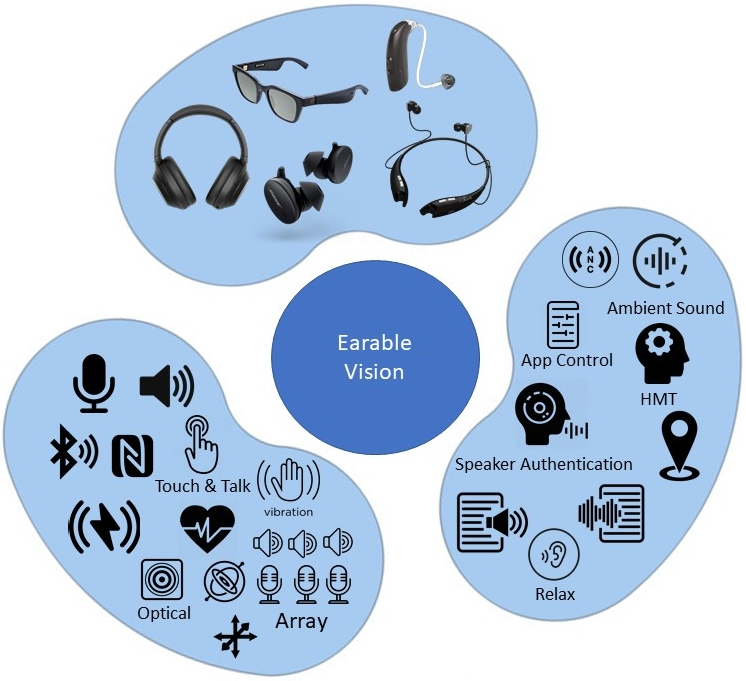
\includegraphics[width=\linewidth]{figs/vision_3.jpg}
    \caption{\small
        Emerging earable devices will be programmable platforms with a rich set
        of sensors and will support a variety of applications.
    }
    \label{fig:earable_vision}
\end{wrapfigure}

There are several signs that earables may become a prominent programmable
computing platform.  First, the current global market for earables is already
over 20 billion dollars and is expected to exceed 90 billion dollars in the
next three years~\cite{}. Second, hardware vendors are already building
earables with increasingly complex sensors (e.g., proximity sensors,
gyroscopes, capacitive sensors, accelerometers, SpO2, EEG, EOG, EMG sensors,
microphone and speaker arrays, etc.) which are being leveraged to support a
wide variety of computing applications~\cite{}.  Third, many earable platforms
are already programmable and increasingly so.  In fact, a large variety of
software applications processing different sensor data are already supported in
many of today's earables~\cite{} or are being explored~\cite{}.  Fourth,
enabling technologies are increasingly production ready.  For example,
transformer networks have enabled super-human performance in natural language
understanding tasks, enabling smart audio interfaces between the earable device
and the user.

Earables as a computing platform may become popular also because acoustic
communication requires much less cognitive re-focus than visual or haptic
communication (e.g., using smartphones)\cite{rethink}. An earable is also a
better platform for sensing and analyzing upper body and head-based data,
compared to a phone or a watch, for example. Furthermore, unlike some other
wearables, most earables (e.g., earphones and hearing aids) already have social
acceptability and wide reach -- computing will simply be piggybacked on
these well-accepted devices.

Another class of sensor data processing that 
mae become 
%has been barely explored in the
mainstream is {\em \olfc{}}.  Smell has always received scant
recognition~\cite{rouby2002olfaction}, and has historically been considered an
inferior sense~\cite{rouby2002olfaction}, in spite of arguably being the most
visceral of senses~\cite{stewart_2022}. Biological understanding of odor has
also been relatively recent~\cite{nobelprize.org_2004}. Previous attempts at \olfc{}, in
the form of e-noses~\cite{karakaya2020electronic}, for example, have seen
limited success~\cite{smith_kiger_2006, platt_1999}, discouraging further
research and adoption; some attempts have indeed been publicly
ridiculed~\cite{smith_kiger_2006}. Finally, odor sensors that \olfc{} would
rely on have historically been highly inaccurate, power hungry, and
slow~\cite{wilson2016recent}; pumps and cartridges required for any odor
synthesis~\cite{olorama_technology, aromajoin_corporation, tillotson2006scent,
amores2017essence, anthrotronix_2019} application have been similarly big,
slow, and power hungry~\cite{mielle2022cold, solis2005fluctuation, maritex}.

\begin{wrapfigure}{r}{0.5\textwidth}
    \centering
    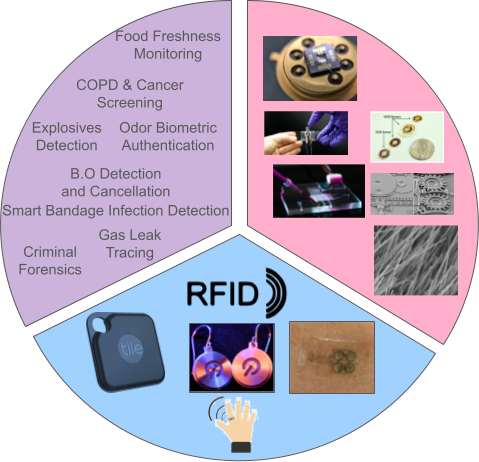
\includegraphics[width=0.7\linewidth]{./figs/odor_vision.png}
    \caption{\small
        An overview of \olfc{} applications,
        form-factors, and sensors \& actuators.
    }
    \label{fig:vision}
\end{wrapfigure}

In spite of the checkered history, we believe that this is a good time to
revisit \olfc{}. A large number of driver applications are emerging that would
require or benefit from \olfc{}. Low cost healthcare (e.g., smart bandages for
infection detection~\cite{derakhshandeh2018smart})  and personal hygiene
applications (body odor detection~\cite{wongchoosuk2009detection, jha2015quick,
jha2016gc, jha2015human}), for example, could benefit greatly when augmented
with odor sensing and synthesis. Second, there have been dramatic recent
advances in odor sensing technology, with some modern odor sensors
demonstrating high accuracy, miniatuarized to the micron scale, and consuming no
more than low tens of \si{\micro\watt} of power
(Fig.~\ref{fig:sensor_timelines}).  There have been similar advances in
NEMS/MEMS-based micropumps and cartridges~\cite{tillotson2006scent}.  Third,
widespread acceptance of sensor, wearable, and xR devices over the last decade,
including recent interest in odor-based wearable~\cite{olorama_technology,
tillotson2006scent, amores2017essence, anthrotronix_2019, peters_2019,
amores2018promoting, bahremand2022smell} and xR~\cite{stewart_2022} devices,
suggests a much easier path of adoption for \olfc{}-based applications than
ever before - overlaid on these devices. This vision of \olfc{} is
depicted in Fig.~\ref{fig:vision} which shows example odor applications, form
factors for \olfc{}-enabled devices, and odor sensors and actuators.




\subsection{Summary of Proposed Research}
\label{ssec:summary}

We ask the question: What kind of programmable hardware will be needed to
support earable computing in the future?  Today's programmable hardware
platforms for earables~\cite{} need to support only limited computation and
sensing and typically consist of either microcontrollers or DSPs or both,
running at low to moderate frequencies. The choice of the earable
microcontrollers (Cortex M4 and M7 cores are popular due to their DSP
extensions) and DSPs (Tensilica HiFi DSPs are popular due to their relatively
low power), their number, and their operating frequencies are limited by the
capacity limitations of today's earable batteries (e.g., AirPods Pro uses a
\SI{45.4}{\milli\ampere\hour}, \SI{3.7}{\volt} battery~\cite{}).

Analogously, we ask the question: What kind of programmable hardware will be needed to
support olfactory computing in the future?
Previous work on \olfc{} has largely focused on sensing applications. A lot of
work exists on commercial and academic e-noses for specific tasks, such as wine
classification~\cite{buratti2004characterization}, evaluating readiness of blue
cheeses~\cite{valente2018cheeses}, assessing seafood freshness~\cite{grassi2022seafood}, and
diagnosing diseases in humans and animals~\cite{gardner2000electronic,
binson2021discrimination, va2021noninvasive, d2010investigation}.  While many
e-noses use electrical resistive sensors, others use gas chromatography-mass
spectrometry~\cite{electronic_sensor_technology, alpha_2018, pan2014early},
which can provide high fidelity chemical detection, but requires a large,
expensive, and power-hungry system, and is thus not suitable for many \olfc{}
applications such as a smart-bandage.
%Fig.~\ref{fig:man_vs_machine} shows the similarities between \olfc{} and
%human olfaction.
Other than sensing, some recent work has begun to re-look at the \textit{odor
synthesis} problem.%\footnote{only 60 years after the disastrous introduction of
%Smell-O-Vision~\cite{smith_kiger_2006}}
Odor synthesis is the creation of
chemicals or chemical mixtures which are perceived to have a certain odor.
There are several contemporary attempts at commercializing odor synthesis,
including a digital scent diffuser - AromaShooter~\cite{aromajoin_corporation},
and wearable devices such as jewelry~\cite{tillotson2006scent} and
headbands~\cite{amores2018promoting}. Odor synthesis has also received interest
within the context of extended reality.  VR SCENT~\cite{olorama_technology}
augments a standard VR system with odor synthesis to assess neuorological
trauma, while The Smell Engine~\cite{bahremand2022smell} is a general odor
synthesis pipeline for VR applications.
No prior work addresses
the organization and design of the olfactory processor itself.


To exploit these opportunities in earable and olfactory processing:
\iffalse
we propose to develop
tools for computer architects, hardware designers, software engineers, and
application developers to better understand sensory computing's software and
hardware ecosystems.  Specifically, the proposed research has two main thrusts,
the first related to \textit{earable computing} and the second to \textit{\olfc}.
The research goals along both thrusts parallel one another:
\fi

1. We will design and publish (open source) benchmark suites for earable and
\olfc{}.  
%Researchers and industry require a benchmark suites
%consisting of representative applications and associated input data.  
Benchmarks
will be written in the C programming language to ensure portability across
existing hardware.  All benchmarks will be published as scalar
and multithreaded workloads (using OpenMP API) to enable benchmarking on single
core, multicore, SMT, and SIMT architectures.

2. We will explore computer architectures for  earable computing and \olfc{}. The exploration will look at both heterogeneous solutions where a system-on-chip targets each computational characteristic with a different component ({\em accelerator}) as well as monolithic solutions where a single processor targets all characteristics. Both classes of solutions could be interesting since both cost and efficiency are concerns.

3. We will prototype an earable computing processor and an \olfc{}
processor, and evaluate the prototypes on the benchmark suites.  This will
give researchers a rigorous performance baseline to compare against, and will
also enable potential technology transfer and commercialization of our sensory
processors.

4. Both earable computing and \olfc{}  may be amenable to computational offloading wherein the
the processor itself is mainly used to collect sensor data (e.g.,
microphones, odor sensors, etc.) and drive actuators (e.g., speakers, lights,
microfluidics, antennae, etc.) while the majority of the computational
requirements of the applications are satisfied on other devices, such
as other wearable or personal devices (smart watch, smart phone, etc.), or
offloaded to cloud or edge server nodes. We will develop offloading-based implementations of applications for different earable and olfactory processor architectures.


\section{Broader Impacts}
\textbf{Artifacts.} The benchmark suites will be
released as open-source software to the community to further academic and
commercial development of earable and olfactory computing systems based on CPU, GPU, DSP, and
spatial computer architectures. We will also release RTL designs and physical design details and scripts corresponding to the chip prototypes of the custom earable
and odor processing computers.

\textbf{Workforce development.}  This work will train several graduate and
undergraduate students an in interdisciplinary area at the intersection of
architecture, application software, and hardware design at both logical and
physical levels.  Graduate students involved in the project will get hands-on
experience with computer architecture, physical design, hardware verification,
and software engineering.

\textbf{Interactions with Industry.}  The PI has active collaborations with
Apple Inc. and Intel, enabling the prototyping of an earable processor and an olfactory processor, and
providing graduate and undergraduate students with mentorship and advising from
industry professionals in hardware design and verification.  These collaborations will be leveraged to enable transfer and potential
commercialization of the earable and odor processing designs developed in this
research.

\textbf{Undergraduate research.}  Undergraduate researchers working with PI
Kumar have published in premiere computer architecture conferences,
including ISCA, HPCA, and DAC.  The HPCA paper was nominated for a Best Paper
Award, and DAC and ISCA papers received significant media coverage.  Several
undergraduate researchers have gone on to join graduate studies at the
University of Illinois, the Massachusetts Institute of Technology, and Carnegie
Mellon University, among others.  The nature of the prototyping aspect of this
project, as well as the large scope of the benchmarking aspect of this project,
will help us engage numerous undergraduate students in research.
%, including the
%design and verification of novel hardware architectures, and the development of
%novel quality of results metrics for the proposed benchmark suite.

\textbf{Curriculum development activities.}  PI Kumar was  awarded the
Ronald W. Pratt Faculty Outstanding Teaching Award and the Stanley H. Pierce
Faculty Award at the University of Illinois for, among other things, innovative
teaching of project-based courses in computer architecture and system design.
He will blend in a discussion of earable and olfactory computing in his graduate and
undergraduate computer architecture classes.  He will also list sensory
computing related projects as project options in the classes, while making
available the proposed  benchmark suites and chip design space
exploration tools to his students.



\section{Proposed Research}
Our proposed research is along two thrusts: earable computing (Section~\ref{sec:tract1})
and \olfc{} (Section~\ref{sec:tract2}).
We have already made progress along both thrusts, including initial analysis
of sensory applications and computational workloads, as well as architectural
exploration and identification of architectures which significantly outperform
existing architectures (Sections~\ref{ssec:prelim1} and \ref{ssec:prelim2}).
As sensory computing is often performed by systems with a wearable form factor,
or as part of a sensor network~\cite{}, we also will explore the benefits
of computational offloading onto other devices such as smart watches, phones,
or cloud platforms.


\section{Thrust 1: Earable Processing}
\label{sec:tract1}
\subsection{Preliminary Results for Thrust 1}
\label{ssec:prelim1}
To understand the hardware requirements for emerging earable applications, we
proposed EarBench, a suite of representative emerging earable applications with
diverse sensor-based inputs and computation requirements
(Table~\ref{tab:earbench}). The EarBench applications have been chosen through
a comprehensive survey of earable applications research~\cite{}, personal
correspondence with domain experts~\cite{}, and profiling of earable
applications to ascertain their execution requirements. We analyzed the
performance of EarBench applications on a spectrum of programmable
microprocessors, including those roughly modeled after ARM Cortex M4 and Cortex
M7 (these cores are a part of several current programmable SoCs). We found that
there is a \(3.97\times\) to \(13.54\times\) performance gap between the
computational needs of EarBench applications and the performance of today's
Cortex M4 and Cortex M7 based programmable earable hardware. More complex
microprocessors (e.g., Cortex A53) can meet the performance requirements of
several EarBench applications, but their high power requirements (e.g.,
\SIrange{276}{339}{\milli\watt} for A53) severely restrict functionality (e.g.,
the number of seconds of audio that can be processed, the number of inferences
and localizations that can be performed, etc. before the battery runs out),
rendering them unacceptable.

Our analysis of EarBench applications also shows that such applications are
dominated by a small number of diverse digital signal processing (DSP) and
machine learning (ML) kernels --- GEMM, GEMV, FFT, bilinear filtering, 1d and
2d convolution, and LU decomposition (Fig.~\ref{fig:earable_kernels}). Any
programmable earable hardware must provide high perfor- mance on these kernels.
We proposed SpEaC --- Spatial Earable Computer --- a coarse-grained
reconfigurable spatial architecture (Figure 3) to target earable applications
efficiently. SpEaC has a fixed-point multiplier and adder tree-based
distribute-then- reduce substrate with support for vectorized complex
operations that energy-efficiently accelerates the earable ML and DSP kernels
and that can be configured for each kernel based on its dataflow. A
tightly-coupled scalar, in-order CPU is responsible for configura- tion and
stream-based programming. The CPU also executes code that does not fit well on
the reconfigurable substrate, including non-multiply or add operations in the
earable DSP kernel code. Unlike recent CGRAs such as SoftBrain\cite{} whose
substrate is designed to support general-purpose computation and lacks direct
support for complex operations, SpEaC substrate is optimized for
energy-efficient execution of the earable kernels at the expense of generality.

Across the kernels, SpEaC outperforms programmable cores modeled after M4, M7,
A53, and HiFi4 DSP by \(99.3\times, 32.5\times, 14.8\times\), and \(9.8\times\)
respectively.

At \SI{63}{\milli\watt} in \SI{28}{\nano\meter}, the energy efficiency benefits
are \(1.55\times, 9.04\times, 68.3\times\), and \(32.7\times\) respectively;
energy efficiency benefits are 15.7× - 1087× over a low power Mali T628 MP6
GPU. Kernel-level benefits also translate into application-level benefits.
SpEaC meets application-level performance requirements of 9 out of 11 EarBench
applications; applications can now run for long periods on an ear- able class
battery.


\begin{wrapfigure}{l}{0.5\textwidth}
  \centering
  % This file was created by tikzplotlib v0.9.8.
\resizebox{\linewidth}{!}{
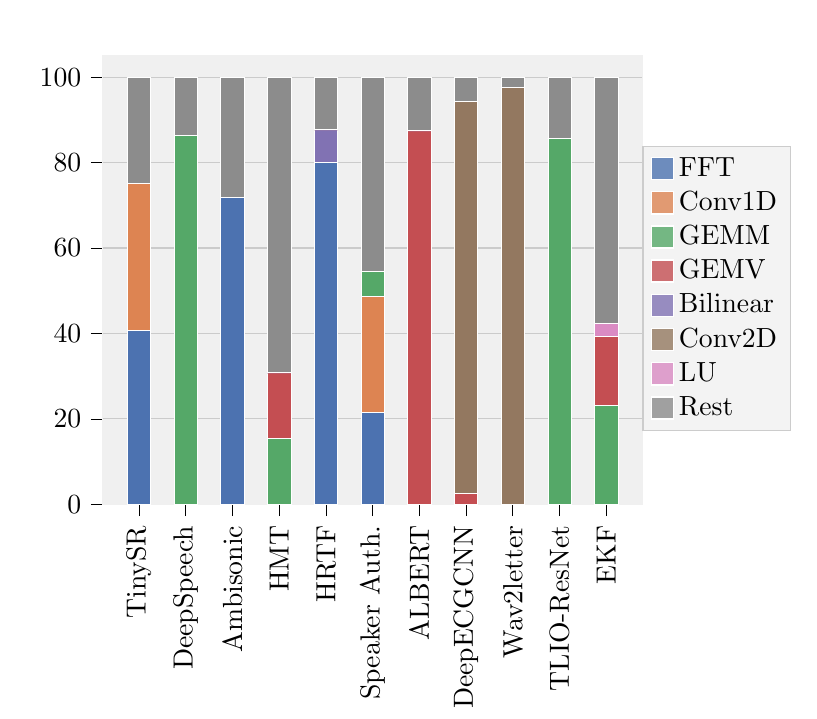
\begin{tikzpicture}

\definecolor{color0}{rgb}{0.298039215686275,0.447058823529412,0.690196078431373}
\definecolor{color1}{rgb}{0.866666666666667,0.517647058823529,0.32156862745098}
\definecolor{color2}{rgb}{0.333333333333333,0.658823529411765,0.407843137254902}
\definecolor{color3}{rgb}{0.768627450980392,0.305882352941176,0.32156862745098}
\definecolor{color4}{rgb}{0.505882352941176,0.447058823529412,0.701960784313725}
\definecolor{color5}{rgb}{0.576470588235294,0.470588235294118,0.376470588235294}
\definecolor{color6}{rgb}{0.854901960784314,0.545098039215686,0.764705882352941}

\begin{axis}[
axis background/.style={fill=white!94.1176470588235!black},
axis line style={white!94.1176470588235!black},
legend cell align={left},
legend style={
  fill opacity=0.8,
  draw opacity=1,
  text opacity=1,
  at={(1,0.8)},
  anchor=north west,
  draw=white!80!black,
  fill=white!94.1176470588235!black
},
tick align=outside,
tick pos=left,
x grid style={white!79.6078431372549!black},
xmin=-0.775, xmax=10.775,
xtick style={color=black},
xtick={0,1,2,3,4,5,6,7,8,9,10},
xticklabel style={rotate=90.0},
xticklabels={
\apptinysr{},
\appdeepspeech{},
\appambisonic{},
\apphmt{},
\apphrtf{},
\appspeakerauthentication{},
\appalbert{},
\appdeepecgcnn{},
\appwavetoletter{},
\appresnet{},
\appekf{}
},
y grid style={white!79.6078431372549!black},
ymajorgrids,
ymin=0, ymax=105,
ytick style={color=black}
]
\draw[draw=white,fill=color0,very thin] (axis cs:-0.25,0) rectangle (axis cs:0.25,40.83);
\addlegendimage{only marks,mark=square*,mark options={mark size=4pt,solid, line width=0.5pt},draw=white,fill=color0,very thin};
\addlegendentry{\kernelfft{}}

\draw[draw=white,fill=color1,very thin] (axis cs:-0.25,40.83) rectangle (axis cs:0.25,75.19);
\addlegendimage{only marks,mark=square*,mark options={mark size=4pt,solid, line width=0.5pt},draw=white,fill=color1,very thin};
\addlegendentry{\kernelconvd{}}

\draw[draw=white,fill=color2,very thin] (axis cs:-0.25,75.19) rectangle (axis cs:0.25,75.19);
\addlegendimage{only marks,mark=square*,mark options={mark size=4pt,solid, line width=0.5pt},draw=white,fill=color2,very thin};
\addlegendentry{\kernelgemm{}}

\draw[draw=white,fill=color3,very thin] (axis cs:-0.25,75.19) rectangle (axis cs:0.25,75.19);
\addlegendimage{only marks,mark=square*,mark options={mark size=4pt,solid, line width=0.5pt},draw=white,fill=color3,very thin};
\addlegendentry{\kernelgemv{}}

\draw[draw=white,fill=color4,very thin] (axis cs:-0.25,75.19) rectangle (axis cs:0.25,75.19);
\addlegendimage{only marks,mark=square*,mark options={mark size=4pt,solid, line width=0.5pt},draw=white,fill=color4,very thin};
\addlegendentry{\kernelbilinear{}}

\draw[draw=white,fill=color5,very thin] (axis cs:-0.25,75.19) rectangle (axis cs:0.25,75.19);
\addlegendimage{only marks,mark=square*,mark options={mark size=4pt,solid, line width=0.5pt},draw=white,fill=color5,very thin};
\addlegendentry{\kernelconvdd{}}

\draw[draw=white,fill=color6,very thin] (axis cs:-0.25,75.19) rectangle (axis cs:0.25,75.19);
\addlegendimage{only marks,mark=square*,mark options={mark size=4pt,solid, line width=0.5pt},draw=white,fill=color6,very thin};
\addlegendentry{\kernellu{}}

\draw[draw=white,fill=white!54.9019607843137!black,very thin] (axis cs:-0.25,75.19) rectangle (axis cs:0.25,100);
\addlegendimage{only marks,mark=square*,mark options={mark size=4pt,solid, line width=0.5pt},draw=white,fill=white!54.9019607843137!black,very thin};
\addlegendentry{\kernelrest{}}

\draw[draw=white,fill=color0,very thin] (axis cs:0.75,0) rectangle (axis cs:1.25,0);
\draw[draw=white,fill=color1,very thin] (axis cs:0.75,0) rectangle (axis cs:1.25,0);
\draw[draw=white,fill=color2,very thin] (axis cs:0.75,0) rectangle (axis cs:1.25,86.37);
\draw[draw=white,fill=color3,very thin] (axis cs:0.75,86.37) rectangle (axis cs:1.25,86.37);
\draw[draw=white,fill=color4,very thin] (axis cs:0.75,86.37) rectangle (axis cs:1.25,86.37);
\draw[draw=white,fill=color5,very thin] (axis cs:0.75,86.37) rectangle (axis cs:1.25,86.37);
\draw[draw=white,fill=color6,very thin] (axis cs:0.75,86.37) rectangle (axis cs:1.25,86.37);
\draw[draw=white,fill=white!54.9019607843137!black,very thin] (axis cs:0.75,86.37) rectangle (axis cs:1.25,100);
\draw[draw=white,fill=color0,very thin] (axis cs:1.75,0) rectangle (axis cs:2.25,71.99);
\draw[draw=white,fill=color1,very thin] (axis cs:1.75,71.99) rectangle (axis cs:2.25,71.99);
\draw[draw=white,fill=color2,very thin] (axis cs:1.75,71.99) rectangle (axis cs:2.25,71.99);
\draw[draw=white,fill=color3,very thin] (axis cs:1.75,71.99) rectangle (axis cs:2.25,71.99);
\draw[draw=white,fill=color4,very thin] (axis cs:1.75,71.99) rectangle (axis cs:2.25,71.99);
\draw[draw=white,fill=color5,very thin] (axis cs:1.75,71.99) rectangle (axis cs:2.25,71.99);
\draw[draw=white,fill=color6,very thin] (axis cs:1.75,71.99) rectangle (axis cs:2.25,71.99);
\draw[draw=white,fill=white!54.9019607843137!black,very thin] (axis cs:1.75,71.99) rectangle (axis cs:2.25,100);
\draw[draw=white,fill=color0,very thin] (axis cs:2.75,0) rectangle (axis cs:3.25,0);
\draw[draw=white,fill=color1,very thin] (axis cs:2.75,0) rectangle (axis cs:3.25,0);
\draw[draw=white,fill=color2,very thin] (axis cs:2.75,0) rectangle (axis cs:3.25,15.47);
\draw[draw=white,fill=color3,very thin] (axis cs:2.75,15.47) rectangle (axis cs:3.25,30.8);
\draw[draw=white,fill=color4,very thin] (axis cs:2.75,30.8) rectangle (axis cs:3.25,30.8);
\draw[draw=white,fill=color5,very thin] (axis cs:2.75,30.8) rectangle (axis cs:3.25,30.8);
\draw[draw=white,fill=color6,very thin] (axis cs:2.75,30.8) rectangle (axis cs:3.25,30.8);
\draw[draw=white,fill=white!54.9019607843137!black,very thin] (axis cs:2.75,30.8) rectangle (axis cs:3.25,100);
\draw[draw=white,fill=color0,very thin] (axis cs:3.75,0) rectangle (axis cs:4.25,80.11);
\draw[draw=white,fill=color1,very thin] (axis cs:3.75,80.11) rectangle (axis cs:4.25,80.11);
\draw[draw=white,fill=color2,very thin] (axis cs:3.75,80.11) rectangle (axis cs:4.25,80.11);
\draw[draw=white,fill=color3,very thin] (axis cs:3.75,80.11) rectangle (axis cs:4.25,80.11);
\draw[draw=white,fill=color4,very thin] (axis cs:3.75,80.11) rectangle (axis cs:4.25,87.76);
\draw[draw=white,fill=color5,very thin] (axis cs:3.75,87.76) rectangle (axis cs:4.25,87.76);
\draw[draw=white,fill=color6,very thin] (axis cs:3.75,87.76) rectangle (axis cs:4.25,87.76);
\draw[draw=white,fill=white!54.9019607843137!black,very thin] (axis cs:3.75,87.76) rectangle (axis cs:4.25,100);
\draw[draw=white,fill=color0,very thin] (axis cs:4.75,0) rectangle (axis cs:5.25,21.597);
\draw[draw=white,fill=color1,very thin] (axis cs:4.75,21.597) rectangle (axis cs:5.25,48.648);
\draw[draw=white,fill=color2,very thin] (axis cs:4.75,48.648) rectangle (axis cs:5.25,54.581);
\draw[draw=white,fill=color3,very thin] (axis cs:4.75,54.581) rectangle (axis cs:5.25,54.581);
\draw[draw=white,fill=color4,very thin] (axis cs:4.75,54.581) rectangle (axis cs:5.25,54.581);
\draw[draw=white,fill=color5,very thin] (axis cs:4.75,54.581) rectangle (axis cs:5.25,54.581);
\draw[draw=white,fill=color6,very thin] (axis cs:4.75,54.581) rectangle (axis cs:5.25,54.581);
\draw[draw=white,fill=white!54.9019607843137!black,very thin] (axis cs:4.75,54.581) rectangle (axis cs:5.25,100);
\draw[draw=white,fill=color0,very thin] (axis cs:5.75,0) rectangle (axis cs:6.25,0);
\draw[draw=white,fill=color1,very thin] (axis cs:5.75,0) rectangle (axis cs:6.25,0);
\draw[draw=white,fill=color2,very thin] (axis cs:5.75,0) rectangle (axis cs:6.25,0);
\draw[draw=white,fill=color3,very thin] (axis cs:5.75,0) rectangle (axis cs:6.25,87.49);
\draw[draw=white,fill=color4,very thin] (axis cs:5.75,87.49) rectangle (axis cs:6.25,87.49);
\draw[draw=white,fill=color5,very thin] (axis cs:5.75,87.49) rectangle (axis cs:6.25,87.49);
\draw[draw=white,fill=color6,very thin] (axis cs:5.75,87.49) rectangle (axis cs:6.25,87.49);
\draw[draw=white,fill=white!54.9019607843137!black,very thin] (axis cs:5.75,87.49) rectangle (axis cs:6.25,100);
\draw[draw=white,fill=color0,very thin] (axis cs:6.75,0) rectangle (axis cs:7.25,0);
\draw[draw=white,fill=color1,very thin] (axis cs:6.75,0) rectangle (axis cs:7.25,0);
\draw[draw=white,fill=color2,very thin] (axis cs:6.75,0) rectangle (axis cs:7.25,0);
\draw[draw=white,fill=color3,very thin] (axis cs:6.75,0) rectangle (axis cs:7.25,2.65);
\draw[draw=white,fill=color4,very thin] (axis cs:6.75,2.65) rectangle (axis cs:7.25,2.65);
\draw[draw=white,fill=color5,very thin] (axis cs:6.75,2.65) rectangle (axis cs:7.25,94.48);
\draw[draw=white,fill=color6,very thin] (axis cs:6.75,94.48) rectangle (axis cs:7.25,94.48);
\draw[draw=white,fill=white!54.9019607843137!black,very thin] (axis cs:6.75,94.48) rectangle (axis cs:7.25,100);
\draw[draw=white,fill=color0,very thin] (axis cs:7.75,0) rectangle (axis cs:8.25,0);
\draw[draw=white,fill=color1,very thin] (axis cs:7.75,0) rectangle (axis cs:8.25,0);
\draw[draw=white,fill=color2,very thin] (axis cs:7.75,0) rectangle (axis cs:8.25,0);
\draw[draw=white,fill=color3,very thin] (axis cs:7.75,0) rectangle (axis cs:8.25,0);
\draw[draw=white,fill=color4,very thin] (axis cs:7.75,0) rectangle (axis cs:8.25,0);
\draw[draw=white,fill=color5,very thin] (axis cs:7.75,0) rectangle (axis cs:8.25,97.76);
\draw[draw=white,fill=color6,very thin] (axis cs:7.75,97.76) rectangle (axis cs:8.25,97.76);
\draw[draw=white,fill=white!54.9019607843137!black,very thin] (axis cs:7.75,97.76) rectangle (axis cs:8.25,100);
\draw[draw=white,fill=color0,very thin] (axis cs:8.75,0) rectangle (axis cs:9.25,0);
\draw[draw=white,fill=color1,very thin] (axis cs:8.75,0) rectangle (axis cs:9.25,0);
\draw[draw=white,fill=color2,very thin] (axis cs:8.75,0) rectangle (axis cs:9.25,85.71);
\draw[draw=white,fill=color3,very thin] (axis cs:8.75,85.71) rectangle (axis cs:9.25,85.71);
\draw[draw=white,fill=color4,very thin] (axis cs:8.75,85.71) rectangle (axis cs:9.25,85.71);
\draw[draw=white,fill=color5,very thin] (axis cs:8.75,85.71) rectangle (axis cs:9.25,85.71);
\draw[draw=white,fill=color6,very thin] (axis cs:8.75,85.71) rectangle (axis cs:9.25,85.71);
\draw[draw=white,fill=white!54.9019607843137!black,very thin] (axis cs:8.75,85.71) rectangle (axis cs:9.25,100);
\draw[draw=white,fill=color0,very thin] (axis cs:9.75,0) rectangle (axis cs:10.25,0);
\draw[draw=white,fill=color1,very thin] (axis cs:9.75,0) rectangle (axis cs:10.25,0);
\draw[draw=white,fill=color2,very thin] (axis cs:9.75,0) rectangle (axis cs:10.25,23.14);
\draw[draw=white,fill=color3,very thin] (axis cs:9.75,23.14) rectangle (axis cs:10.25,39.36);
\draw[draw=white,fill=color4,very thin] (axis cs:9.75,39.36) rectangle (axis cs:10.25,39.36);
\draw[draw=white,fill=color5,very thin] (axis cs:9.75,39.36) rectangle (axis cs:10.25,39.36);
\draw[draw=white,fill=color6,very thin] (axis cs:9.75,39.36) rectangle (axis cs:10.25,42.47);
\draw[draw=white,fill=white!54.9019607843137!black,very thin] (axis cs:9.75,42.47) rectangle (axis cs:10.25,100);
\end{axis}

\end{tikzpicture}
} % resizebox

  \caption{\small Constituent kernels of EarBench applications.}
  \label{fig:kernels_breakdown}
\end{wrapfigure}


\begin{table}[]
\label{tab:earbench}
\caption{EarBench: Inputs, outputs and timing requirements.}
\tiny
\begin{tabular}{ll}
\toprule
Applications    & Inputs / Outputs / Timing Requirements  \\ \midrule
tinySR          & 1s audio /
Small vocabulary English words
/ real time ($\leq \SI{1}{\second}$)   \\
DeepSpeech      & 5s audio /
English text
/ real time ($\leq \SI{1}{\second}$)   \\
Ambisonic-2/6/8     & 10s audio /
Binauralized audio
/ real time ($\leq \SI{1}{\second}$)   \\
HMT-1           & IMU@\SI{100}{\hertz} /
dead-reckoned location of the user
/  $\leq \SI{1}{\second}$             \\
HMT-10          & IMU@\SI{1}{\kilo\hertz} /
dead-reckoned location of the user
/ $\leq \SI{1}{\second}$               \\
HRTF - 2/6/8    &  8sec audio / binauralized audio /   $\leq \SI{1}{\second}$ \\
Speaker Auth.   & 1s audio /
Classifies the speaker as one of the 10 authorized speakers,\\
& or as unauthorized
/ real time ($\leq \SI{1}{\second}$)    \\
ALBERT          & question (10 words) /
start\_logits: the logits of being \\
& the start of the answer of each position
end\_logits: the logits of being \\
& the end of the answer of each position.
/  $\leq \SI{3}{\second}$\\
DeepECGCNN      & 9s ECG signal  /
Four output classes 1) Normal sinus rhythm, 2) Arrhythmic, \\
& 3) Other kind
of rhythm,
4) Very noisy,
/ 9s                    \\
Wave2Letter     &  MFCC with input tensor share (1, 296, 39)
/ Tensor of time and class probability of shape \\
& (1, 1, 148, 29)
/ real time ($\leq \SI{1}{\second}$)  \\
TLIO-1DResNet18 & IMU@200HZ/
Two 3D vectors, the displacement estimates and their \\
& uncertainties
/ $\leq \SI{0.1}{\second}$/inference \\
EKF & IMU data 75k samples / Orientation of IMU /  $\leq \SI{1}{\second}$\\
\bottomrule
\end{tabular}
\label{tab:requirements}
\end{table}

To construct EarBench, a suite of representative emerging earable applications,
we conducted a comprehensive survey of earable applications research and
practice~\cite{}, including over 50 papers on http://esense.io, and interviewed
three earable computing domain experts [69]. We observed that most research and
commercial earable computing applications fall into one of four categories: (1)
Human-Machine Interface (HMI) applications that allow the earable user to
interact with the device (and vice-versa). In the absence of traditional
interfaces (e.g., keyboard, mouse, touchscreen), interactions are typically via
sound and taps. (2) Audio applications that decode, manipulate, and playback
audio data streams (e.g., phone calls, podcasts, acoustic augmented reality
(AAR)). (3) Analytics applications, such as ECG monitors, that are
computation-heavy but should ideally execute locally on the earable device.
Finally, (4) Spatial Awareness applications that localize the user, their
movements, head gestures, etc. for applications in AR/VR, gaming, location-
specific alerts, etc. These spatial tracking applications are often
characterized by sensor fusion engines, and are thus assigned to a separate
category. To have a representative, but diverse suite, we then selected from
each category 2-4 applications with different computational requirements, as
determined by profiling (Table~\ref{tab:earbench_metrics}), and diverse
sensor-based inputs. Diversity was considered also in terms of underlying
algorithms (e.g., DSP vs ML, RNN vs CNN vs BERT) and use cases (e.g.,
authentication vs recognition, classifi- cation vs NLP, tracking vs
localization).

\begin{table}[]
\caption{\small EarBench: Execution characteristics.
\label{tab:earbench_metrics}
`RSS' and `WSS' are resident and working set sizes in \si{\mega\byte}. `Comp.',
`Cond.', `Uncond.', and `Mem.' columns correspond to the percent of dynamic
instructions categorized as computation, conditional branching,
unconditional branching, and memory accessing, respectively. `Inst. Count'
is the dynamic instruction count (in millions). `FPA2M' is the ratio of
floating point arithmetic to bytes of memory accessed (Wav2letter uses
integer arithmetic only).
}
\resizebox{1.0\columnwidth}{!}{%
\begin{tabular}{lllllllll}
\toprule
            & RSS    & WSS   & Inst. Count & Comp.  & Cond.  & Uncond. & Mem.  & FPA2M \\ \midrule
TinySR      & 1.56   & 0.07  & 313         & 36.5   & 4.4    & 2.2     & 56.9  & 0.518 \\
HMT         & 1.77   & $<0.01$ & 14          & 49.2   & 4.4    & 3.4     & 42.7  & 0.878 \\
Ambisonic   & 6.82   & 5.42  & 2,795       & 51.9   & 7.2    & 1.4     & 39.5  & 1.27  \\
SpeakerAuth & 6.40   & 3.62  & 1,520       & 26.6   & 15.4   & 1.5     & 56.4  & 1.07  \\
HRTF        & 8.95   & 3.97  & 2,712       & 59.4   & 12.6   & 1.3     & 26.7  & 1.49  \\
DeepECGCNN  & 1084   & 1071  & 3,295       & 72.5   & 14.4   & 0.01    & 13.1  & 1.00  \\
DeepSpeech  & 226    & 195   & 3,486       & 30.6   & 3.3    & 16.8    & 49.3  & 1.07  \\
TLIO        & 39.8   & 0.5   & 87          & 69.0   & 17.4   & 0.37    & 13.1  & 1.00  \\
Wav2Letter  & 29.7   & 28.1  & 1,077       & 79.4   & 2.01   & 0.06    & 18.4  & (N/A) \\
EKF         & 8.9    & 0.63  & 1,351       & 44.9   & 14.0   & 4.76    & 36.2  & 0.760 \\
ALBERT      & 773    & 767   & 15,213      & 73.7   & 1.77   & 0.18    & 24.3  & 1.00  \\ \bottomrule
\end{tabular}}

\end{table}

Fig.~\ref{fig:earable_results} presents speed-up results for simulations of
SpEaC against cores modeled after Cortex M4 (s\_180), Cortex M7 (ss\_480) and
Cortex A53 (ss\_1000) in the gem5 architectural simulator, as well as against
measured results of a HiFi4 DSP.  Across the computation kernels, SpEaC is 5.1
to \(195\times\) faster than s\_180, 1.2 to \(35\times\) faster than ss\_1000,
and 3.8 to \(12.5\times\) faster than the HiFi4 DSP. SpEaC outperforms ss\_1000
by an average of \(11\times\) and outperforms the HiFi4 DSP by an average of
\(6.57\times\).

\begin{wrapfigure}{L}{0.5\textwidth}
    \centering
    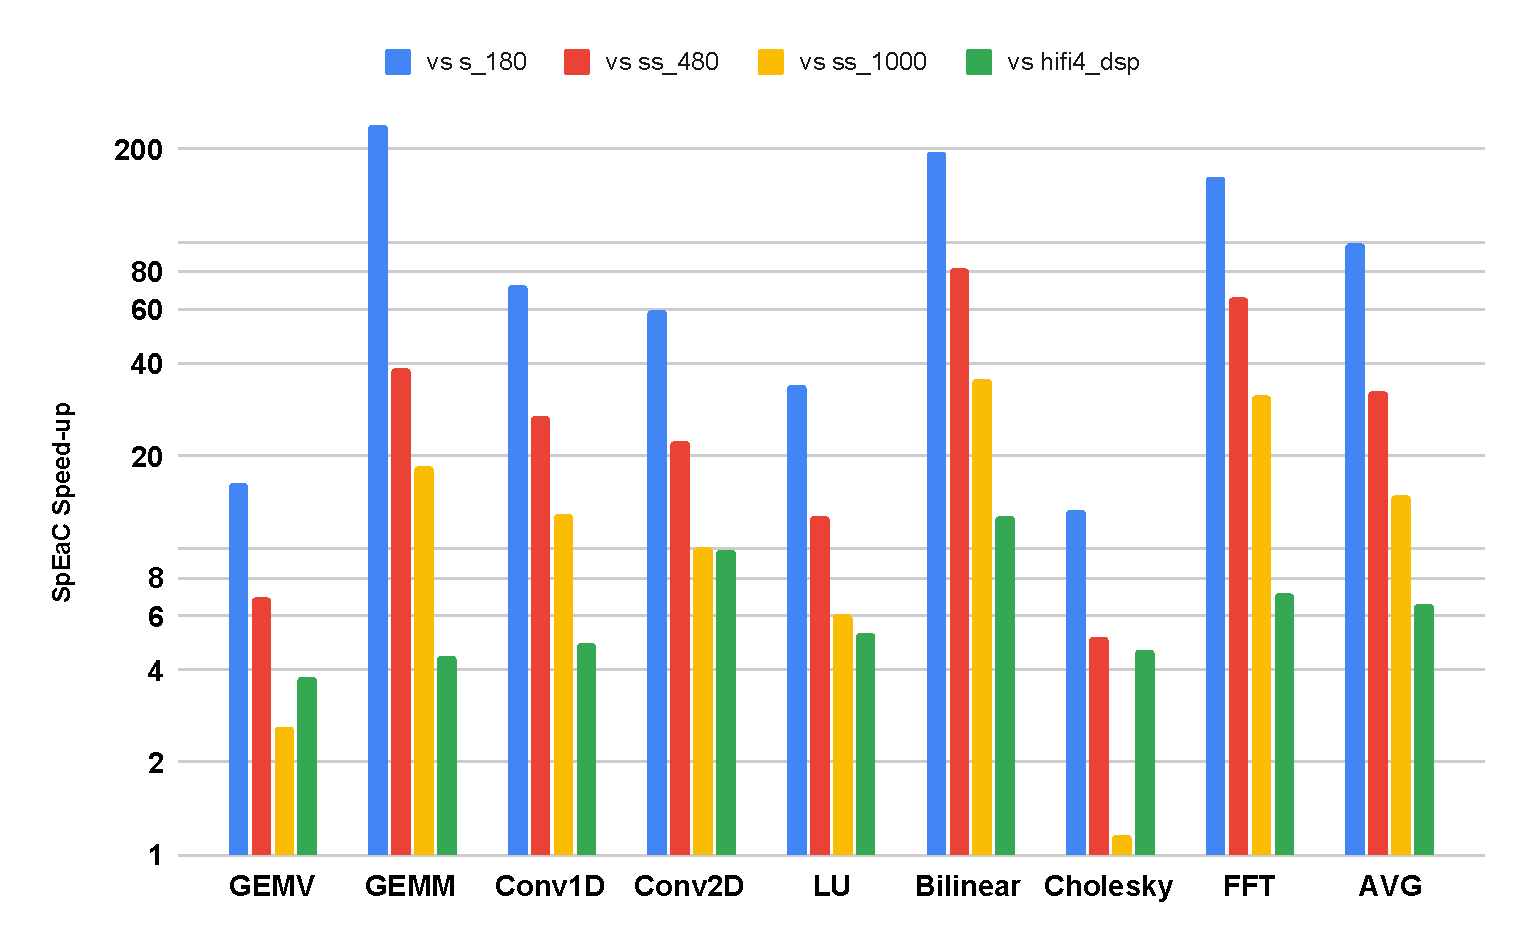
\includegraphics[width=\linewidth]{./figs/speedup.pdf}
    \caption{\small
    Speed-up of SpEaC over modeled cores.
    }
    \label{fig:earable_results}
\end{wrapfigure}

\begin{wrapfigure}{L}{0.5\textwidth}
    \centering
    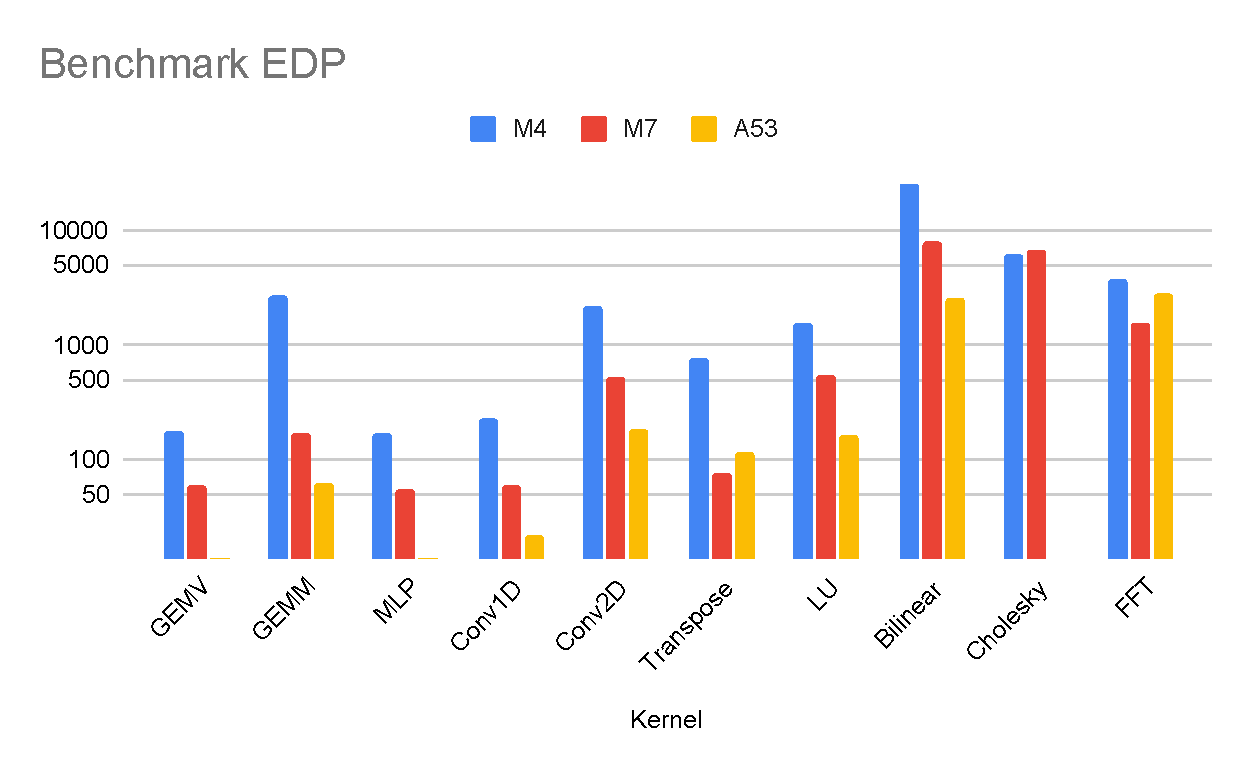
\includegraphics[width=\linewidth]{./figs/edp.pdf}
    \caption{\small
    Energy improvement from SpEaC over modeled cores.
    }
    \label{fig:earable_edp}
\end{wrapfigure}

Fig.~\ref{fig:earable_edp} shows the energy benefit of SpEaC relative to the
baseline cores. The benefits are up to \(160\times\) compared against the
microprocessors, and up to over \(42\times\) compared to the DSP.

The percentage of total energy consumption consumed by adders and multiplier
functional units is < 20\% for each kernel. The high overhead of control and
data movement reinforce the importance of minimizing the CGRA network costs
(using a tree, for example), the use of specialized FUs (using only fixed point
adders and multipliers on the substrate, for example), and the associated
memory system. Using kernel speed-up values from simulation, and with the
kernel-breakdown of Fig.~\ref{fig:earable_results}, we estimate the application
level speed-up and energy benefits of SpEaC. Compared against ss\_1000,
significant application level speed-ups are significant: \(3.3\times\) for
Deep- Speech and Ambisonic, \(6.6\times\) to \(9.6\times\) for HRTF audio,
\(3.6\) for the ResNet, \(2.2\times\) for ALBERT, \(6.4\times\) for DeepECGCNN,
and \(8.3\times\) for WaveToLetter. In fact, these speed-ups are achieved
despite ss\_1000 consuming \(2\times\) to \(2.5\times\) more power than SpEaC.
These speed-ups are large enough to allow SpEaC to meet the application-level
requirements of all applications, except ALBERT and EKF. Recall
that s\_180, ss\_480, and ss\_1000 met requirements for 0, 2, and 6 applications
respecitively.

To understand the system-level impact of SpEaC, we also consider non-compute
components. Table 5 lists power and latency of several non-compute components.
The latency overhead of the non-compute components is much smaller than the
estimated latency of Earbench applications on SpEaC. We estimate that, compared
to s\_180, ss\_480 and ss\_1000, the speedup of SpEaC on-average across all
EarBench applications is only reduced by 0.67\%, 0.51\% and 0.33\% respectively,
when the latency of all the non-compute components in Table 5 is added. We
similarly estimated (Figure 6) the number of times different EarBench
applications whose performance requirements are met by the SpEaC can be run on
the SpEaC given the energy budget of a \SI{45.4}{\milli\ampere\hour},
\SI{3.7}{\volt} battery.


\begin{wrapfigure}{L}{0.5\textwidth}
    \centering
    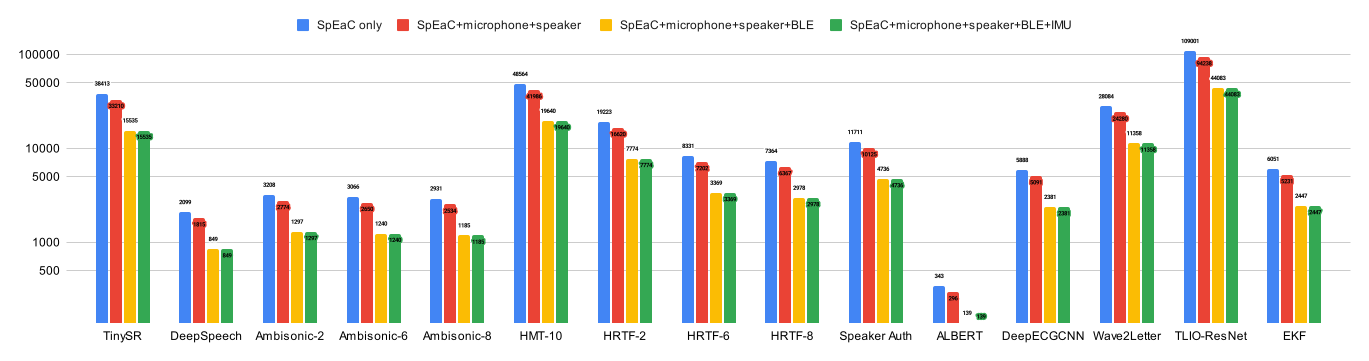
\includegraphics[width=\linewidth]{./figs/speakandsensors.png}
    \caption{\small
    Number of runs on SpEaC on a \SI{45.4}{\milli\ampere\hour}, \SI{3.7}{\volt}
    battery.
    }
    \label{fig:earable_edp}
\end{wrapfigure}

Our results show that even when the microphone, speaker, BLE and IMU sensor are
simultaneously consuming battery energy, the EarBench applications can still
run hundreds of times. E.g. DeepSpeech on 5s audio can run 849 times before
battery needs recharging; this corresponds to large-vocabulary speech
recognition for 1.14 hours. To validate our estimates, we ported TinySR to
SpEaC, implementing the FFT component on the CGRA. Based on TinySR’s estimates,
we had expected to see a \(2.7\times\) speed-up on SpEaC. Simulation of the SpEaC port
of TinySR showed a \(2.5\times\) speed-up, a −7\% error versus our analytic estimate. A
\(2.5\times\) performance improvement on TinySR also corresponds to a
\(5.8\times\) improvement in energy efficiency, and a \(14.4\times\)
improvement in EDP.



\subsection{Research Goals}
\label{ssec:research1}

Of course, to build earable computing systems, we must understand and analyze
characteristics of earable applications.  In this work, through a survey of
research literature and recent practice, and conversations with earable computing domain experts,
%and our own experience with building and prototyping application specific
%systems, 
we will first identify a set of computation tasks that may be common across
a variety of earable applications.  We will then identify, through
a survey of papers discussing implementations of these tasks, a set of
algorithms that often underpin these tasks.  We will then understand through
profiling-based measurements the computational characteristics of these
algorithms.  An understanding of these
characteristics can be used to build and optimize earable computing systems for different
system-level constraints.


\begin{table}[]
\centering
\label{tab:earbench_metrics}
\caption{Representative earable applications: Inputs, outputs and timing requirements.}
\tiny
\begin{tabular}{ll}
\toprule
Applications    & Inputs / Outputs / Timing Requirements  \\ \midrule
tinySR          & 1s audio /
Small vocabulary English words
/ real time ($\leq \SI{1}{\second}$)   \\
DeepSpeech      & 5s audio /
English text
/ real time ($\leq \SI{1}{\second}$)   \\
Ambisonic-2/6/8     & 10s audio /
Binauralized audio
/ real time ($\leq \SI{1}{\second}$)   \\
HMT-1           & IMU@\SI{100}{\hertz} /
dead-reckoned location of the user
/  $\leq \SI{1}{\second}$             \\
HMT-10          & IMU@\SI{1}{\kilo\hertz} /
dead-reckoned location of the user
/ $\leq \SI{1}{\second}$               \\
HRTF - 2/6/8    &  8sec audio / binauralized audio /   $\leq \SI{1}{\second}$ \\
Speaker Auth.   & 1s audio /
Classifies the speaker as one of the 10 authorized speakers,\\
& or as unauthorized
/ real time ($\leq \SI{1}{\second}$)    \\
ALBERT          & question (10 words) /
start\_logits: the logits of being \\
& the start of the answer of each position
end\_logits: the logits of being \\
& the end of the answer of each position.
/  $\leq \SI{3}{\second}$\\
DeepECGCNN      & 9s ECG signal  /
Four output classes 1) Normal sinus rhythm, 2) Arrhythmic, \\
& 3) Other kind
of rhythm,
4) Very noisy,
/ 9s                    \\
Wave2Letter     &  MFCC with input tensor share (1, 296, 39)
/ Tensor of time and class probability of shape \\
& (1, 1, 148, 29)
/ real time ($\leq \SI{1}{\second}$)  \\
TLIO-1DResNet18 & IMU@200HZ/
Two 3D vectors, the displacement estimates and their \\
& uncertainties
/ $\leq \SI{0.1}{\second}$/inference \\
EKF & IMU data 75k samples / Orientation of IMU /  $\leq \SI{1}{\second}$\\
\bottomrule
\end{tabular}
\end{table}

As preliminary analysis,
we conducted a comprehensive survey of earable applications research and
practice~\cite{waverly, nuraphone, scribd, bible, peckham_sarkar_2019},
including over 50 papers on http://esense.io, and interviewed three earable
computing domain experts. We observed that most research and commercial earable
computing applications fall into one of four categories: (1) Human-Machine
Interface (HMI) applications that allow the earable user to interact with the
device (and vice-versa). In the absence of traditional interfaces (e.g.,
keyboard, mouse, touchscreen), interactions are typically via sound and taps.
(2) Audio applications that decode, manipulate, and playback audio data streams
(e.g., phone calls, podcasts, acoustic augmented reality (AAR)). (3) Analytics
applications, such as ECG monitors, that are computation-heavy but should
ideally execute locally on the earable device. Finally, (4) Spatial Awareness
applications that localize the user, their movements, head gestures, etc. for
applications in AR/VR, gaming, location- specific alerts, etc. These spatial
tracking applications are often characterized by sensor fusion engines, and are
thus assigned to a separate category. To have a representative, but diverse
suite, we then selected from each category 2-4 applications with different
computational requirements, as determined by profiling
(Table~\ref{tab:earbench_metrics}), and diverse sensor-based inputs. Diversity
was considered also in terms of underlying algorithms (e.g., DSP vs ML, RNN vs
CNN vs BERT) and use cases (e.g., authentication vs recognition, classification
vs NLP, tracking vs localization).

We will continue the analysis to finalize the list of representative
computational tasks and then build EarSuite --- the first earable computing
benchmark suite --- by porting all benchmark code to C and OpenMP, designing
representative inputs for each benchmark, and providing baselines on existing
systems.
    %We will enable
    %EarSuite evaluations for heterogeneous systems --- both heterogeneous
    %SoCs, as well as multi-chip and even multi-device systems.  
EarSuite --- software, data, \& build scripts --- as well as executable
binaries for major platforms --- will be published under an open source license
in order to enable commercial and academic research in earable computing.
%    EarBench will consist of a diverse and representative set of current and
 %   future earable computing applications.  
 Data inputs will be drawn from real world inputs (e.g., measured microphone,
 accelerometer, \& ECG data), popular queries to current question-answering
 systems (e.g., Alexa, Google Assistant, etc.).

EarSuite will be published with a CMake based build system.  As CMake is an
open-source, cross platform build automation tool targeting all major operating
systems, and since nearly all computer architectures have open source or
proprietary C compilers, researchers will be able to get EarSuite running on a
wide variety of systems quickly and easily. For major architectures (e.g.,
ARMv7, ARMv8, x86\_64, i686, etc.), we will provide prebuilt EarSuite binaries.

The next goal is to explore computer architectures for earable processing.
Naturally, the question arises --
%Are today's hardware platforms not good enough to support earable applications? Second, 
what are the key computational characteristics that any earable computing
platform should target?
% We analyze the EarBench suite to identify the key
% computation kernels in earable  applications.
Figure~\ref{fig:kernels_breakdown} shows the performance breakdown of some
representative applications across constituent kernels on a single Cortex A72
(profiling was performed on Raspberry Pi 4).  Applications were compiled with
gcc 9.2 and rustc 1.5 with `O3' optimizations (which include SIMD
auto-vectorization).
 
 
 
\begin{figure}[h]
  \centering
%   \includegraphics[height=\linewidth,
%   width=1.1\linewidth]{images/kernelsbreakdown.png}
  
    \scalebox{0.65}{% This file was created by tikzplotlib v0.9.8.
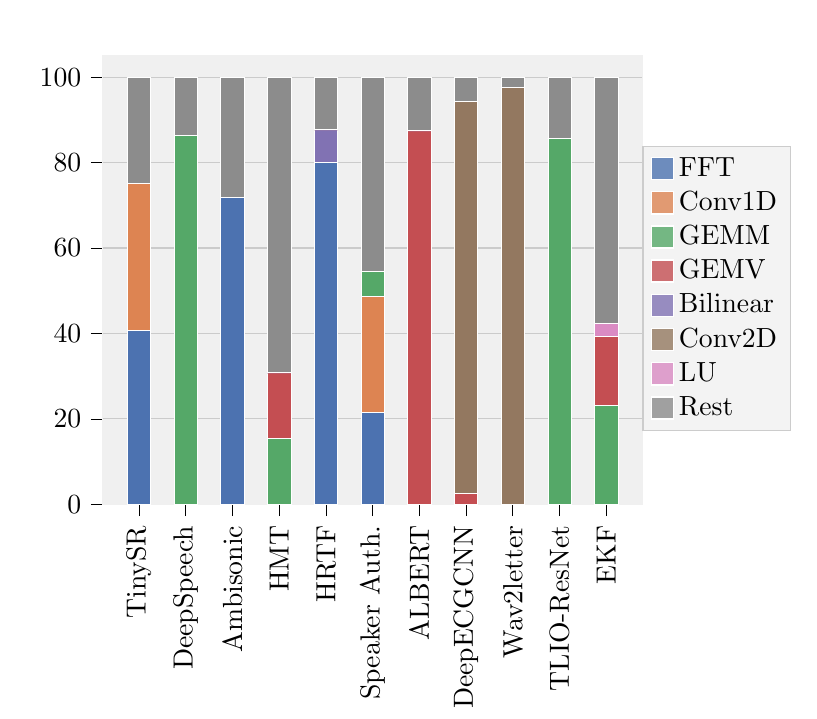
\begin{tikzpicture}

\definecolor{color0}{rgb}{0.298039215686275,0.447058823529412,0.690196078431373}
\definecolor{color1}{rgb}{0.866666666666667,0.517647058823529,0.32156862745098}
\definecolor{color2}{rgb}{0.333333333333333,0.658823529411765,0.407843137254902}
\definecolor{color3}{rgb}{0.768627450980392,0.305882352941176,0.32156862745098}
\definecolor{color4}{rgb}{0.505882352941176,0.447058823529412,0.701960784313725}
\definecolor{color5}{rgb}{0.576470588235294,0.470588235294118,0.376470588235294}
\definecolor{color6}{rgb}{0.854901960784314,0.545098039215686,0.764705882352941}

\begin{axis}[
axis background/.style={fill=white!94.1176470588235!black},
axis line style={white!94.1176470588235!black},
legend cell align={left},
legend style={
  fill opacity=0.8,
  draw opacity=1,
  text opacity=1,
  at={(1,0.8)},
  anchor=north west,
  draw=white!80!black,
  fill=white!94.1176470588235!black
},
tick align=outside,
tick pos=left,
x grid style={white!79.6078431372549!black},
xmin=-0.775, xmax=10.775,
xtick style={color=black},
xtick={0,1,2,3,4,5,6,7,8,9,10},
xticklabel style={rotate=90.0},
xticklabels={
\apptinysr{},
\appdeepspeech{},
\appambisonic{},
\apphmt{},
\apphrtf{},
\appspeakerauthentication{},
\appalbert{},
\appdeepecgcnn{},
\appwavetoletter{},
\appresnet{},
\appekf{}
},
y grid style={white!79.6078431372549!black},
ymajorgrids,
ymin=0, ymax=105,
ytick style={color=black}
]
\draw[draw=white,fill=color0,very thin] (axis cs:-0.25,0) rectangle (axis cs:0.25,40.83);
\addlegendimage{only marks,mark=square*,mark options={mark size=4pt,solid, line width=0.5pt},draw=white,fill=color0,very thin};
\addlegendentry{\kernelfft{}}

\draw[draw=white,fill=color1,very thin] (axis cs:-0.25,40.83) rectangle (axis cs:0.25,75.19);
\addlegendimage{only marks,mark=square*,mark options={mark size=4pt,solid, line width=0.5pt},draw=white,fill=color1,very thin};
\addlegendentry{\kernelconvd{}}

\draw[draw=white,fill=color2,very thin] (axis cs:-0.25,75.19) rectangle (axis cs:0.25,75.19);
\addlegendimage{only marks,mark=square*,mark options={mark size=4pt,solid, line width=0.5pt},draw=white,fill=color2,very thin};
\addlegendentry{\kernelgemm{}}

\draw[draw=white,fill=color3,very thin] (axis cs:-0.25,75.19) rectangle (axis cs:0.25,75.19);
\addlegendimage{only marks,mark=square*,mark options={mark size=4pt,solid, line width=0.5pt},draw=white,fill=color3,very thin};
\addlegendentry{\kernelgemv{}}

\draw[draw=white,fill=color4,very thin] (axis cs:-0.25,75.19) rectangle (axis cs:0.25,75.19);
\addlegendimage{only marks,mark=square*,mark options={mark size=4pt,solid, line width=0.5pt},draw=white,fill=color4,very thin};
\addlegendentry{\kernelbilinear{}}

\draw[draw=white,fill=color5,very thin] (axis cs:-0.25,75.19) rectangle (axis cs:0.25,75.19);
\addlegendimage{only marks,mark=square*,mark options={mark size=4pt,solid, line width=0.5pt},draw=white,fill=color5,very thin};
\addlegendentry{\kernelconvdd{}}

\draw[draw=white,fill=color6,very thin] (axis cs:-0.25,75.19) rectangle (axis cs:0.25,75.19);
\addlegendimage{only marks,mark=square*,mark options={mark size=4pt,solid, line width=0.5pt},draw=white,fill=color6,very thin};
\addlegendentry{\kernellu{}}

\draw[draw=white,fill=white!54.9019607843137!black,very thin] (axis cs:-0.25,75.19) rectangle (axis cs:0.25,100);
\addlegendimage{only marks,mark=square*,mark options={mark size=4pt,solid, line width=0.5pt},draw=white,fill=white!54.9019607843137!black,very thin};
\addlegendentry{\kernelrest{}}

\draw[draw=white,fill=color0,very thin] (axis cs:0.75,0) rectangle (axis cs:1.25,0);
\draw[draw=white,fill=color1,very thin] (axis cs:0.75,0) rectangle (axis cs:1.25,0);
\draw[draw=white,fill=color2,very thin] (axis cs:0.75,0) rectangle (axis cs:1.25,86.37);
\draw[draw=white,fill=color3,very thin] (axis cs:0.75,86.37) rectangle (axis cs:1.25,86.37);
\draw[draw=white,fill=color4,very thin] (axis cs:0.75,86.37) rectangle (axis cs:1.25,86.37);
\draw[draw=white,fill=color5,very thin] (axis cs:0.75,86.37) rectangle (axis cs:1.25,86.37);
\draw[draw=white,fill=color6,very thin] (axis cs:0.75,86.37) rectangle (axis cs:1.25,86.37);
\draw[draw=white,fill=white!54.9019607843137!black,very thin] (axis cs:0.75,86.37) rectangle (axis cs:1.25,100);
\draw[draw=white,fill=color0,very thin] (axis cs:1.75,0) rectangle (axis cs:2.25,71.99);
\draw[draw=white,fill=color1,very thin] (axis cs:1.75,71.99) rectangle (axis cs:2.25,71.99);
\draw[draw=white,fill=color2,very thin] (axis cs:1.75,71.99) rectangle (axis cs:2.25,71.99);
\draw[draw=white,fill=color3,very thin] (axis cs:1.75,71.99) rectangle (axis cs:2.25,71.99);
\draw[draw=white,fill=color4,very thin] (axis cs:1.75,71.99) rectangle (axis cs:2.25,71.99);
\draw[draw=white,fill=color5,very thin] (axis cs:1.75,71.99) rectangle (axis cs:2.25,71.99);
\draw[draw=white,fill=color6,very thin] (axis cs:1.75,71.99) rectangle (axis cs:2.25,71.99);
\draw[draw=white,fill=white!54.9019607843137!black,very thin] (axis cs:1.75,71.99) rectangle (axis cs:2.25,100);
\draw[draw=white,fill=color0,very thin] (axis cs:2.75,0) rectangle (axis cs:3.25,0);
\draw[draw=white,fill=color1,very thin] (axis cs:2.75,0) rectangle (axis cs:3.25,0);
\draw[draw=white,fill=color2,very thin] (axis cs:2.75,0) rectangle (axis cs:3.25,15.47);
\draw[draw=white,fill=color3,very thin] (axis cs:2.75,15.47) rectangle (axis cs:3.25,30.8);
\draw[draw=white,fill=color4,very thin] (axis cs:2.75,30.8) rectangle (axis cs:3.25,30.8);
\draw[draw=white,fill=color5,very thin] (axis cs:2.75,30.8) rectangle (axis cs:3.25,30.8);
\draw[draw=white,fill=color6,very thin] (axis cs:2.75,30.8) rectangle (axis cs:3.25,30.8);
\draw[draw=white,fill=white!54.9019607843137!black,very thin] (axis cs:2.75,30.8) rectangle (axis cs:3.25,100);
\draw[draw=white,fill=color0,very thin] (axis cs:3.75,0) rectangle (axis cs:4.25,80.11);
\draw[draw=white,fill=color1,very thin] (axis cs:3.75,80.11) rectangle (axis cs:4.25,80.11);
\draw[draw=white,fill=color2,very thin] (axis cs:3.75,80.11) rectangle (axis cs:4.25,80.11);
\draw[draw=white,fill=color3,very thin] (axis cs:3.75,80.11) rectangle (axis cs:4.25,80.11);
\draw[draw=white,fill=color4,very thin] (axis cs:3.75,80.11) rectangle (axis cs:4.25,87.76);
\draw[draw=white,fill=color5,very thin] (axis cs:3.75,87.76) rectangle (axis cs:4.25,87.76);
\draw[draw=white,fill=color6,very thin] (axis cs:3.75,87.76) rectangle (axis cs:4.25,87.76);
\draw[draw=white,fill=white!54.9019607843137!black,very thin] (axis cs:3.75,87.76) rectangle (axis cs:4.25,100);
\draw[draw=white,fill=color0,very thin] (axis cs:4.75,0) rectangle (axis cs:5.25,21.597);
\draw[draw=white,fill=color1,very thin] (axis cs:4.75,21.597) rectangle (axis cs:5.25,48.648);
\draw[draw=white,fill=color2,very thin] (axis cs:4.75,48.648) rectangle (axis cs:5.25,54.581);
\draw[draw=white,fill=color3,very thin] (axis cs:4.75,54.581) rectangle (axis cs:5.25,54.581);
\draw[draw=white,fill=color4,very thin] (axis cs:4.75,54.581) rectangle (axis cs:5.25,54.581);
\draw[draw=white,fill=color5,very thin] (axis cs:4.75,54.581) rectangle (axis cs:5.25,54.581);
\draw[draw=white,fill=color6,very thin] (axis cs:4.75,54.581) rectangle (axis cs:5.25,54.581);
\draw[draw=white,fill=white!54.9019607843137!black,very thin] (axis cs:4.75,54.581) rectangle (axis cs:5.25,100);
\draw[draw=white,fill=color0,very thin] (axis cs:5.75,0) rectangle (axis cs:6.25,0);
\draw[draw=white,fill=color1,very thin] (axis cs:5.75,0) rectangle (axis cs:6.25,0);
\draw[draw=white,fill=color2,very thin] (axis cs:5.75,0) rectangle (axis cs:6.25,0);
\draw[draw=white,fill=color3,very thin] (axis cs:5.75,0) rectangle (axis cs:6.25,87.49);
\draw[draw=white,fill=color4,very thin] (axis cs:5.75,87.49) rectangle (axis cs:6.25,87.49);
\draw[draw=white,fill=color5,very thin] (axis cs:5.75,87.49) rectangle (axis cs:6.25,87.49);
\draw[draw=white,fill=color6,very thin] (axis cs:5.75,87.49) rectangle (axis cs:6.25,87.49);
\draw[draw=white,fill=white!54.9019607843137!black,very thin] (axis cs:5.75,87.49) rectangle (axis cs:6.25,100);
\draw[draw=white,fill=color0,very thin] (axis cs:6.75,0) rectangle (axis cs:7.25,0);
\draw[draw=white,fill=color1,very thin] (axis cs:6.75,0) rectangle (axis cs:7.25,0);
\draw[draw=white,fill=color2,very thin] (axis cs:6.75,0) rectangle (axis cs:7.25,0);
\draw[draw=white,fill=color3,very thin] (axis cs:6.75,0) rectangle (axis cs:7.25,2.65);
\draw[draw=white,fill=color4,very thin] (axis cs:6.75,2.65) rectangle (axis cs:7.25,2.65);
\draw[draw=white,fill=color5,very thin] (axis cs:6.75,2.65) rectangle (axis cs:7.25,94.48);
\draw[draw=white,fill=color6,very thin] (axis cs:6.75,94.48) rectangle (axis cs:7.25,94.48);
\draw[draw=white,fill=white!54.9019607843137!black,very thin] (axis cs:6.75,94.48) rectangle (axis cs:7.25,100);
\draw[draw=white,fill=color0,very thin] (axis cs:7.75,0) rectangle (axis cs:8.25,0);
\draw[draw=white,fill=color1,very thin] (axis cs:7.75,0) rectangle (axis cs:8.25,0);
\draw[draw=white,fill=color2,very thin] (axis cs:7.75,0) rectangle (axis cs:8.25,0);
\draw[draw=white,fill=color3,very thin] (axis cs:7.75,0) rectangle (axis cs:8.25,0);
\draw[draw=white,fill=color4,very thin] (axis cs:7.75,0) rectangle (axis cs:8.25,0);
\draw[draw=white,fill=color5,very thin] (axis cs:7.75,0) rectangle (axis cs:8.25,97.76);
\draw[draw=white,fill=color6,very thin] (axis cs:7.75,97.76) rectangle (axis cs:8.25,97.76);
\draw[draw=white,fill=white!54.9019607843137!black,very thin] (axis cs:7.75,97.76) rectangle (axis cs:8.25,100);
\draw[draw=white,fill=color0,very thin] (axis cs:8.75,0) rectangle (axis cs:9.25,0);
\draw[draw=white,fill=color1,very thin] (axis cs:8.75,0) rectangle (axis cs:9.25,0);
\draw[draw=white,fill=color2,very thin] (axis cs:8.75,0) rectangle (axis cs:9.25,85.71);
\draw[draw=white,fill=color3,very thin] (axis cs:8.75,85.71) rectangle (axis cs:9.25,85.71);
\draw[draw=white,fill=color4,very thin] (axis cs:8.75,85.71) rectangle (axis cs:9.25,85.71);
\draw[draw=white,fill=color5,very thin] (axis cs:8.75,85.71) rectangle (axis cs:9.25,85.71);
\draw[draw=white,fill=color6,very thin] (axis cs:8.75,85.71) rectangle (axis cs:9.25,85.71);
\draw[draw=white,fill=white!54.9019607843137!black,very thin] (axis cs:8.75,85.71) rectangle (axis cs:9.25,100);
\draw[draw=white,fill=color0,very thin] (axis cs:9.75,0) rectangle (axis cs:10.25,0);
\draw[draw=white,fill=color1,very thin] (axis cs:9.75,0) rectangle (axis cs:10.25,0);
\draw[draw=white,fill=color2,very thin] (axis cs:9.75,0) rectangle (axis cs:10.25,23.14);
\draw[draw=white,fill=color3,very thin] (axis cs:9.75,23.14) rectangle (axis cs:10.25,39.36);
\draw[draw=white,fill=color4,very thin] (axis cs:9.75,39.36) rectangle (axis cs:10.25,39.36);
\draw[draw=white,fill=color5,very thin] (axis cs:9.75,39.36) rectangle (axis cs:10.25,39.36);
\draw[draw=white,fill=color6,very thin] (axis cs:9.75,39.36) rectangle (axis cs:10.25,42.47);
\draw[draw=white,fill=white!54.9019607843137!black,very thin] (axis cs:9.75,42.47) rectangle (axis cs:10.25,100);
\end{axis}

\end{tikzpicture}

}
  \caption{\small Constituent kernels of representative earable applications.}
%  \vspace{-7mm}
    \label{fig:kernels_breakdown}
\end{figure}


Figure~\ref{fig:kernels_breakdown} shows that earable applications are
built out of a small number of computationally intensive DSP and ML
kernels.  At first glance, this commonality of kernels in applications
%crossing four taxonomic categories, with
across  a wide range of use-cases (e.g., audio playback, text processing,
heart-rate monitoring, speech processing, etc.) may seem surprising.
However, note that these applications are implemented broadly using techniques from digital signal processing and machine learning; 
%DSP and ML computation are well-known to both be dominated by a small number of computation kernels and share  computation kernels between them~\cite{narayan2019novel}. 
%\nathan{
Machine learning and DSP kernels have similar computation.
A neural network consists of an alternating sequence of linear transformations and non-linear activation functions. Computing the action of a linear transformation, $W$, on an input vector, $a$, is given by $b = Wa$.  Given a choice of basis, $W$ and $a$ can be expressed in matrix form, and computing the $i$'th output of $b$ is
\begin{equation}
    b_i = \sum_{n=0}^{N-1} a_jW_{ij}.
\end{equation}
Similarly, computing the $N$-point discrete Fourier transform (DFT) of a real or complex vector, $x$, is given by the linear transformation $X = Wx$, and $W_{nk} = e^{-i2\pi/N}$ is an element of the order $N$ subgroup of the unit circle group.
Thus, the `frequency-domain' output
\begin{equation}
   X[k] = \sum_{n=0}^{N-1} x[n] W_{nk}
\end{equation}
is remarkably similar to the core computation of a neural network.
Two factors complicate using a substrate optimized for ML kernels to be used for DSP kernels and vice versa. First, neural networks typically are real-valued, while DFT is complex valued.  Second, symmetries in the DFT's transformation enable a `fast' $O(n\log n)$ Fourier transform by recursively subdividing the $N$-point DFT into smaller and smaller sub-blocks.  Similarly, neural networks often exploit symmetries of their own to greatly reduce required computation and data movement by using convolution layers.
Despite these complications, striking similarities remain.  Both DFT and neural network computations are made up of real-valued multiplications followed by additions/subtractions, and in both the number of multiplications needed is nearly identical to the number of additions/subtractions needed. This suggests that an efficient processor architecture for earable applications is a neural network accelerator that is augmented with support for complex processing and that can be reconfigured to support different dataflows for the different ML and DSP kernels. 

Furthermore, since the dataflows of dot-product and complex multiplication, the key subcomputations of neural networks and FFT, respectively, consist of scattering
data streams to multiplication units, followed by reduction (dot-product) and gathering into an output stream (complex multiplication), an architecture which enables scatter-multiply-reduce and scatter-multiply-gather is needed
(Figure~\ref{fig:complex-vs-dot}).
High bandwidth tree-structures for both the scatter network, and for the reduction/gather network should enable efficient computation of machine learning and DSP workloads.

\begin{figure}[htbp]
 \centering
   \subfloat{
   {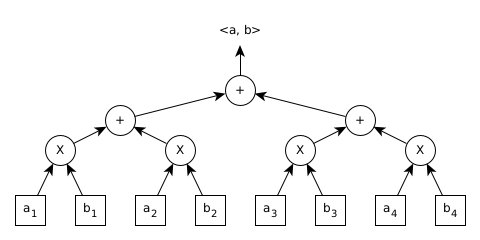
\includegraphics[width=0.48\linewidth]{dot_prod_dataflow.png}}
   }
   \subfloat{
   {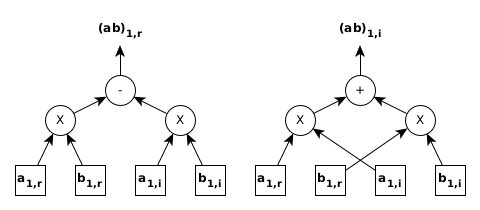
\includegraphics[width=0.48\linewidth]{complex_multiply_dataflow.png}}
   }
   %\label{fig:complex-vs-dot}
   \caption{
   \small
   Dataflows for dot-product (left) and complex multiplication (right).
 }
% \vspace{-5mm}
 \label{fig:complex-vs-dot}
 %\label{fig:vm-configs}
\end{figure}




Many classes of programmable hardware, such as GPUs and DSPs, already
accelerate a variety of DSP and ML kernels. However, they draw high power
(e.g., \SI{234}{\milli\watt} for HiFi4 DSP, 1.8W for Mali T628 MP6 GPU vs tens
of \si{\milli\watt}s required for earable hardware) due to their excessive
generality. 
For example, GPUs use expensive floating point
arithmetic (vs fixed point arithmetic that may be adequate for earable
computing kernels), general-purpose microarchitecture (earable applications may largely need only a tree of adders and multipliers customized to the earable ML/DSP kernels), and
dedicated graphics pipelines (that unnecessarily contribute static power in
context of earable computing). 

ML accelerators are not a good fit either
since it is unclear how to map earable DSP kernels such as LU, Bilinear, Cholesky, and FFT on such hardware (due to lack of
support for non-matrix computation, vectorized complex operations, or non-multiply or add
operations, for example). 

\begin{figure}[h]
  \centering
  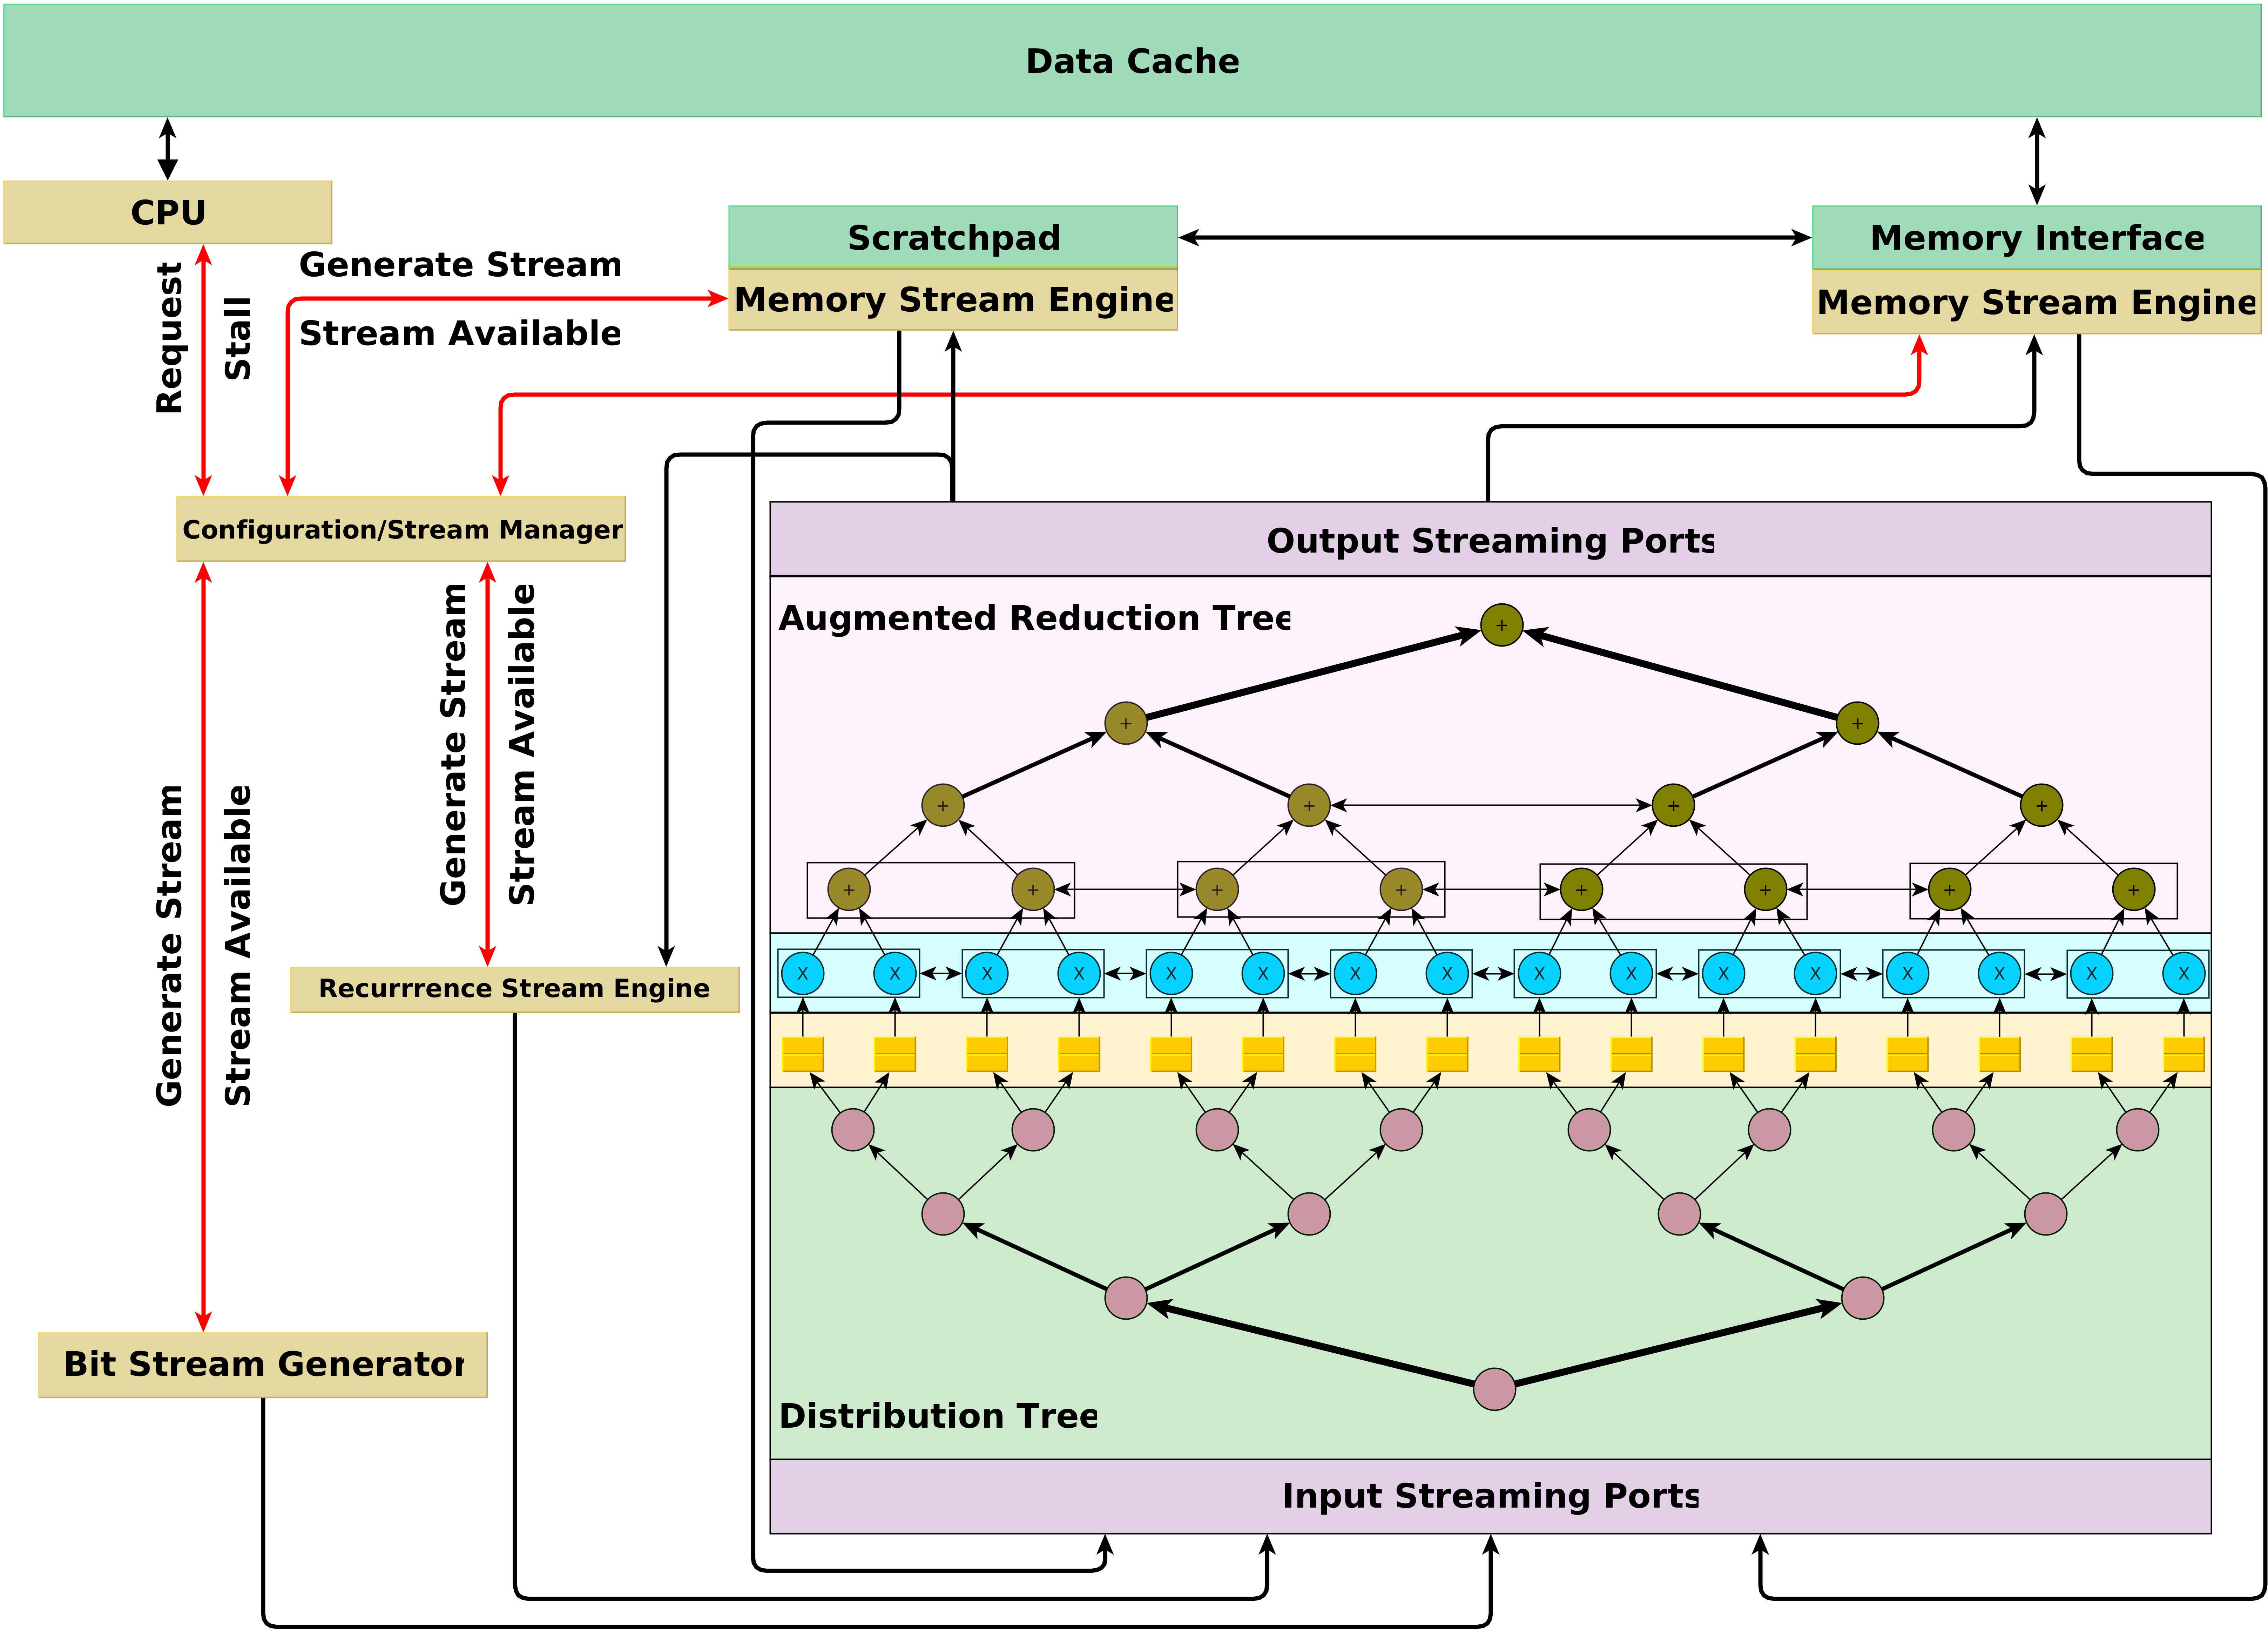
\includegraphics[width=0.48\textwidth]{arch.png}
  %\includesvg[height=\linewidth,width=\textwidth]{images/arch.svg}
  \caption{
  \small
  Architecture of \arch{}.}
  \label{fig:earable_arch}
\end{figure}

We will use EarSuite to drive a design space exploration of computer
architectures for earable processing. An example computer architecture (that we
have preliminarily explored~\cite{bleier2022rethinking}) is  a
stream-programmed~\cite{nowatzki2017stream} coarse-grained reconfigurable
spatial architecture (Figure~\ref{fig:earable_arch}) whose computation
substrate consists of a set of  adders and multipliers (since earable
applications are dominated by inner-product-based computation).
A fat distribution
tree~\cite{leiserson1985fat}  feeds the multiplier units.  The products
of the multiplier units are forwarded to the adders organized in an `augmented
reduction tree', which allows a single tree to perform multiple inner
products concurrently, or to be time-multiplexed to perform a large inner-product across multiple cycles.
The final few adder units are equipped
with accumulators to enable computation of multiple inner-products in parallel. The accumulators may be configured to output either
the accumulated value, $x$, or $\max{\{0, x\}}$, such that the architecture supports
either linear or reLU activation functions.  Max-pooling
layers is supported through the reduction tree by allowing the adder units to also perform
comparison operations.
 The architecture  uses  32-bit fixed-point arithmetic since high quality audio
often has a 24-bit depth, while 16-bit fixed-point arithmetic would %necessarily
lower audio quality. 
Furthermore, since FFT is a key computational kernel in earable application, the
functional units support vectorized complex operations. To enable 
multiplication of complex numbers, two adjacent multipliers form a pair to create a  {\em
logical vector multiplier}.
%which perform complex multiplication and
%addition on streams of complex numbers (in array-of-structs form). In order to
%support this the vectorized PEs 
Each logical vector multiplier can be configured to either perform a 2x32 bit
multiplication or a 2x32 bit multiplication in which one of the 64-bit inputs'
top and bottom 32-bits are swapped. Also, since $i^2 = -1$, the real component
of the complex product is produced by computing the difference of two of the
partial products while the imaginary component is produced by computing the sum
of the other two partial products. To support this,  adjacent adders in level 3
of the tree form  \textit{logical vector adders}. The `left' adder in a logical
vector adder can be configured to perform subtraction as well as addition. The
control core executes code that does not fit well on the reconfigurable
substrate, including non-multiply or add operations in the DSP kernel code
(e.g., square-root and divide operations in LU and Cholesky).

There are several other computer architectures possible as well. One
possibility is to support multiple fixed function accelerators on the earable
SoC each targeting a different set of kernels. For example, an SoC with a CPU,
an ML accelerator, and an FFT accelerator looks attractive for our
applications. However, there are several disadvantages of such an approach.
One, the field of earable computing is relatively new and algorithms are still
evolving. Any system with fixed functions ASICs may become obsolete quickly.
Second,  a collection of special purpose accelerators will fail to provide the
requisite performance for kernels that do not map well to an existing
accelerator. For example, LU, Bilinear, and Cholesky cannot be mapped directly
on an ML accelerator or an FFT accelerator and will need to be run on the CPU
at high performance cost. Similarly, a given kernel may not fit its fixed
function accelerator well depending on the input. For example, FFT size in
tinySR, depends on input audio length and, for our microphone input, varies
from 32-point to 1024-point, HRTF calls a 4096-point FFT, Ambisonic uses a 512
or 1024-point FFT, etc. Many FFT accelerators are optimized for a specific
size~\cite{fft01} and will not run other FFTs of other sizes
efficiently~\cite{fft02}. Nevertheless, a heterogeneous system has benefits in
terms of reusability and cost. We will compare the spatial approaches against
heterogeneous approaches.

We will also prototype and test an earable computer in TSMC \(\leq
\SI{65}{\nano\meter}\) technology. The candidate design, the spatial
architecture described above, shows significant performance and energy
improvement over existing hardware systems used in today's earable computers.
Prototyping sub-objectives include physical design of the architecture to
minimize energy, including design and placement of multiple power and clock
domains, integration of the architecture with commercially licensable SRAMs to
minimize cost, and design for test, chip tape-out, and packaging for workforce
development.  Multiple power domains are used as the architecture is a
heterogeneous system (control core and reconfigurable substrate), and thus
power gating can be used to reduce static power consumption. Similarly, clock
and voltage scaling can be used minimize energy or power consumption when one
or more of the architecture's components has performance slack available.
Although we have a preliminary architecture, a careful exploration would be
needed to determine the optimal choice of operating points.   Similarly,
testing sub-objectives include earable system design and PCB design, porting
EarSuite applications to the chip, and collecting measured EarSuite results.
System design will incorporate multiple earable sensors (e.g., microphone
arrays, inertial motion units), actuators (e.g., speakers, antennae), and a
hardware debug system. Porting EarSuite applications to the chip requires
annotating the EarSuite C code with pragmas which enable the architecture's
compiler to automatically generate configurations and data streams for its
spatial accelerator. PI Kumar is experienced in digital design, chip design,
tape-out and testing, and runs an undergraduate course in which students design
and tape-out processors which are manufactured by TSMC and then tested at UIUC
campus. His research group also participates in Intel's Chip Design Challenge,
in manufacturing RISC-V processors in Intel's \SI{16}{\nano\meter} technology.
The research group has also recently taped out several flexible
chips~\cite{bleier2022flexicores, Bleier_2023}.


\begin{figure}[htbp]
  \centering
    \subfloat{
        {\includesvg[width=0.48\linewidth]{kernels.svg}}
        }
    \subfloat{
        {\includesvg[width=0.48\linewidth]{applications.svg}}
    }
    \caption{ Communication energy of BLE transceiver when inputs and outputs
    are transmitted over BLE for remote compute offloading, normalized with
    respect to the energy consumed when kernels and applications are
    computed locally.}
  \label{fig:ble}
\end{figure}

A natural question comes up: whether to offload compute to 
mobile device (using BLE, for example) - this will involve sending inputs and outputs over the communication protocol - or compute locally on an earable processor? 
 Communication can be expensive. \cite{ble} claims that it takes $8usec$ to communicate one byte of data over BLE whereas the TX power of BLE is 84mW and RX power is 66mW. 
 %We used power and communication latency numbers from \cite{ble} along with the input and output sizes of our kernels and applications and computed the
%energy consumed by the BLE transceiver.
Figure~\ref{fig:ble}-a shows the 
communication energy of BLE transceiver normalized with respect to the energy consumed by the above proposed spatial architecture when we run the kernels locally on the architecture. Our results show that 
computing kernels locally is on average $\approx4OOM$ more energy efficient compared to communicating inputs/outputs over BLE. This is not surprising since BLE
%although BLE is low power protocol, it 
consumes significant amount of energy ($\approx\SI{0.7}{\micro\joule\per\byte}$~\cite{ble}) when sending large matrices, which are common inputs to our kernels, due to its long communication latency.
Similarly, figure~\ref{fig:ble}-b shows the 
communication energy of BLE transceiver normalized with respect to the energy consumed by the spatial architecture when we run the entire application locally. The results show that 
for compute intensive applications, e.g. Albert, it is more energy efficient to offload compute to remote device,
whereas for all other applications 
computing applications locally is more energy efficient than offloading the compute to remote device over BLE.
On average computing locally  is $\approx12.7\times$ more energy efficient across applications we considered compared to communicating inputs/outputs over BLE. 
%Another possibility is to offload computation to a remote, non-earable device. However, this leads to concerns about energy (since energy of transmitting
%    data wirelessly via BLE is orders of magnitude greater than transmitting
%    data to/from local memory, 
Other than energy benefits, local computation may often be preferred also for improved 
%as well as 
latency, privacy, and usability (since a remote device may not always be available or accessible).

At the same time, applications such as Albert which have high computation and
memory requirements may need to be offloaded to a remote device both for energy
and capability reasons. We will analyze both proposed hardware and existing
earable hardware in a heterogeneous, networked computational settings, in which
computation can be offloaded from the earable device onto a number of other
devices, including smart watches,  smart phones, and high performance cloud
systems. We will use HPVM~\cite{ejjeh2022hpvm} for distributed implementation
of the EarSuite benchmarks. The distributed implementations will be open
sourced and released publicly.
%\end{enumerate}


\section{Thrust 2: Odor Processing}
\label{sec:tract2}
\subsection{Preliminary Results for Thrust 2}
\label{ssec:prelim2}
\begin{table}[]
\caption{Examples of \olfc{} applications and their constraints.}
\label{tab:applications}
\begin{adjustbox}{max width=\linewidth}
\begin{tabular}{@{}ll@{}}
\toprule
\textbf{Application}              & \textbf{Constraints}     \\ \midrule
Food Freshness Monitoring         & \(\leq\si{\milli\watt}\), lifetime of hours - months \\
Food Spoilage Detection           & \(\leq\si{\milli\watt}\), lifetime of hours - months \\
Personal Hygiene Monitoring       & low \si{\milli\watt}, lifetime of $\leq$ day         \\
Wearable Body Odor Detection      & low \si{\milli\watt}, lifetime of days               \\
Odor Biometric Authentication     & lifetime of months-years                             \\
Odor Biometric Forensics          & field deployable \& single use                       \\
Smart-Bandage infection detection & \(<\si{\milli\watt}\), lifetime of hours - days      \\
Air and water quality monitoring  & \(<\si{\milli\watt}\), lifetime of months - years    \\
Dangerous compound detection      & lifetime of days-years                               \\
Explosive detection               & lifetime of days-years                               \\
Gas Leak Tracing                  & requires spatial dispersed sensors, lifetime of minutes to hours \\
Odor Cancellation                 & requires odor synthesis  \\
Bespoke clothing deoderization    & requires odor synthesis  \\
Olfactory enabled xR              & requires odor synthesis \\
Food \& Scent recommendation      &                          \\
COPD \& Lung Cancer Screening     &                          \\
    \bottomrule
\end{tabular}
\end{adjustbox}
\end{table}


To build \olfc{} systems, we analyzed the computational tasks underpinning
odor-based applications. To identify a set of computation tasks that may be
common across a variety of odor-based applications, we surveyed 25 papers
published in last 10 years on odor-based applications in
Table~\ref{tab:applications} - at least one paper on each application was
found. We identified the computational task(s) each paper was focused on. We
also surveyed 10 odor-based electronic products in last five years and
identified the corresponding computational task(s). Finally, we interviewed
three olfaction experts and asked them for a list of computational tasks. We
then created a list of tasks that appeared in at least two of the above three
lists.

\textbf{Odor Processing Tasks.}
The tasks in our finalized list are odor localization, odor classification,
odor authentication, odor similarity, active odor cancellation, odor
pleasantness estimation, and odor demixing.

Odor classification, as the name suggests, is the task associated with
identifying the source of an odor.  Odor classification uses machine learning
and statistical techniques to map chemical sensor readings to source
odorants~\cite{kaeppler2013odor, husni2017odor}. Odor classification has many
commercial, industrial, agricultural, medical, and security applications,
including food and beverage monitoring for spoilage and
quality~\cite{yu2008quality, pan2014early, chen2013classification,
yu2008identification, yu2009identification}, alcohol~\cite{
    zhang2021channel,buratti2004characterization,shi2019deep},
    fruits~\cite{pan2014early, chen2018characterization, chen2018development,
    du2019ripeness, rasekh2021nose, wu2017sensor}, cooking
    oils~\cite{karami2020application, teixeira2021application,
    rasekh2021classification}, meats and seafood~\cite{panigrahi2006design,
    wijaya2019noise, wijaya2021dwtlstm, aunsa2021electronic,
    grassi2022seafood}, dairy~\cite{yang2021application, labreche2005shelf},
    and vinegar~\cite{li2022physicochemical, anklam1998characterisation}).
    Industrial applications include environmental monitoring for air quality
    and air pollution estimation~\cite{caron2019identification,
    szulczynski2017different, tacstan2019real, de2008tinynose}, while
    agriculture applications include waste-water monitoring and forestry
    applications~\cite{wilson2013diverse, blanco2018development,
    lagod2019application, dewettinck2001electronic}. Medical applications for
    odor classification have begun to emerge, including hygiene
    monitoring~\cite{lorwongtragool2014novel}, diagnosis of lung diseases such
    as COPD and lung cancer~\cite{gardner2000electronic, va2021noninvasive,
    binson2021discrimination, d2010investigation}. Security applications
    include and explosive device detection~\cite{brudzewski2012metal,
    lopez2017electronic, sun2013liquid}. Odor classification is performed with
    a variety of machine learning and statistical analysis techniques such as
    principal component analysis (PCA), support vector machines (SVM),
    artificial neural networks (ANN), and K-Means cluster analysis (KMeans).

Biometric authentication using odor, or, odor authentication, is the olfactory
equivalent of fingerprint, facial, iris, or voice authentication techniques
which are currently in vogue on mobile devices~\cite{stokkenes2016biometric}.
Individual humans have an identifiable scent due to genetic and environmental
factors~\cite{penn2007individual}, and many studies have shown successful
discrimination of individuals' body odor using chemical sensor
data~\cite{wongchoosuk2009detection, jha2015quick, jha2016gc}. Several odor
authentication schemes have been proposed~\cite{yang2018human,
shu2014identification}. Odor authentication is similar to odor classification
in that it uses machine learning to classify a body odor as authenticated or
non-authenticated, however, it typically uses a dictionary of known odors.
Similar to other biometric authentication techniques, odor authentication
consists of first extracting features from chemical sensor data, often using
parametric machine learning learning techniques, and then comparing those
features to a user dictionary. Thus, new authenticated users can be enrolled
and old users removed without needing to retrain a new model from the ground
up~\cite{wong2001enhanced}. Algorithms in odor authentication include PCA, SVM,
ANN, K-Means, and KNN.

In the odor similarity task, the goal is to estimate the odor similarity of two
different chemical mixtures.  Traditionally, this has been done by first
identifying the chemical structure of the mixtures' constituent chemicals via
\gcms{} (however, it can also be done with sensor data).  These
chemical structures are then mapped to fixed length vectors from an inner
product space, and then the mixtures are represented by weighted sums of the
constituent chemical vectors.  Finally, the similarity of the two chemicals is
scored based on the angle between the two vectors
(AngleDist)~\cite{snitz2013predicting}.

Active odor cancellation is the olfactory equivalent of active noise
cancellation.  Active odor cancellation attempts to `block out' one or more
malodors in an environment by \textit{adding} odors which cancel the malodor,
rendering it as olfactory white noise~\cite{varshney2014active}.
The algorithm which determines how much of each odor to add to the environment
consists of solving a quadratic program which, in many cases, is convex. As
such, gradient descent based optimizers may be used to find local, and often,
global solutions to the optimization problem.

The pleasantness of an odor is highly dependent on the physical properties of
the odorant molecular structure~\cite{arshamian2022perception}. As such, odor
pleasantness estimation is assigning a value (either numeric or categorical) to
a chemical corresponding to its predicted pleasantness.  This has been achieved
using PCA and SVM~\cite{li2018accurate, li2020perception, shang2017machine}.

Odorants exist in mixtures, including time-evolving mixtures, yet often only
one chemical odorant is of interest.  Odor demixing is the task which isolates
the signal corresponding to the chemical of interest.  
This can be achieved
using \gcms{}, however, as \gcms{} requires a large laboratory set-up, and
takes twenty or more minutes to perform. %different techniques are required when
%working with low-power chemical sensors. 
There have been a number of works
which attempt to tackle this problem in context of low-power chemical sensors~\cite{maho2021real, victor2014combining,
fonollosa2014chemical}, but odor demixing remains a largely unexplored \olfc{}
task. However, odor demixing has been studied in biological olfactory systems,
and several studies have proposed biology inspired compressive sensing, which
enables reconstructing sparse signals from many fewer samples than is typically
required (e.g., in an audio setting, from samples taken below the Nyquist
rate)~\cite{fornasier2015compressive}. Compressive sensing, namely, orthogonal
matching pursuit (OMP), has been shown to be useful in the olfactory domain
since individual odors are sparse within the large space in which an odor can
be represented.

Odor localization is the task of identifying the source location of an
odorant `plume' within an environment.  Odor localization is efforts are
exacerbated by the turbulent nature gas plumes which result in non-convex
distributions of the odarant plume with local maxima, which limit the
applicability of gradient based methods.  As such, biology inspired methods, as
well as probabilistic methods such as particle filtering are commonly used in
conjunction with a model of plume dynamics~\cite{vickers2000mechanisms}.
While odor localization
%is unique
%among the tasks in that it 
is typically performed by either a mobile field robot~\cite{chen2019odor}, or
by a distributed sensor network~\cite{hayes2002distributed}, as odor
localization benefits from taking chemical readings in multiple locations
throughout the environment, we also consider future applications where a
wearable aids a moving human or an animal in identifying an odor source (gas
leak or fire source, for example).
%Analogously, consider triangulating a radio signal broadcast
%location --- this task is much easier with receivers in multiple locations than
%with only a single radio receiver.  Indeed, with only a single, fixed chemical
%sensor, it is exceedingly difficult to determine if a faint signal is due
%to a strong odorant source far away, or a weak odorant source nearby.

\textbf{Algorithms}
To analyze a computer architecture's performance on \olfc{} workloads, a
diverse and representative collection of \olfc{} algorithms underpinning the
odor computational tasks is needed. To that end, nine benchmark kernels
were selected using the following selection methodology:
\begin{itemize}
    \item Select a keyword for each given \olfc{} task.
    \item Collect the top 50 most relevant papers returned by Google Scholar
          for the selected keyword.
    \item Sort the papers by the number of citations per year.
    \item Take up to the top ten relevant papers from this list.
    \item Any algorithm that is used two or more times in these papers is added
          to the list of algorithms for the corresponding task.
    \item Algorithmic metaparameters (e.g., neural network architectures,
          dimensionality, etc.) are taken by using the most heavyweight version
          of the algorithms found in the search (see Table~\ref{tab:kernels}).
          In one case, metaparameters
          are determined by memory availability on the baseline architecture
          (i.e., the number of particles used in particle filtering).
\end{itemize}


\begin{wrapfigure}{l}{0.5\linewidth}
    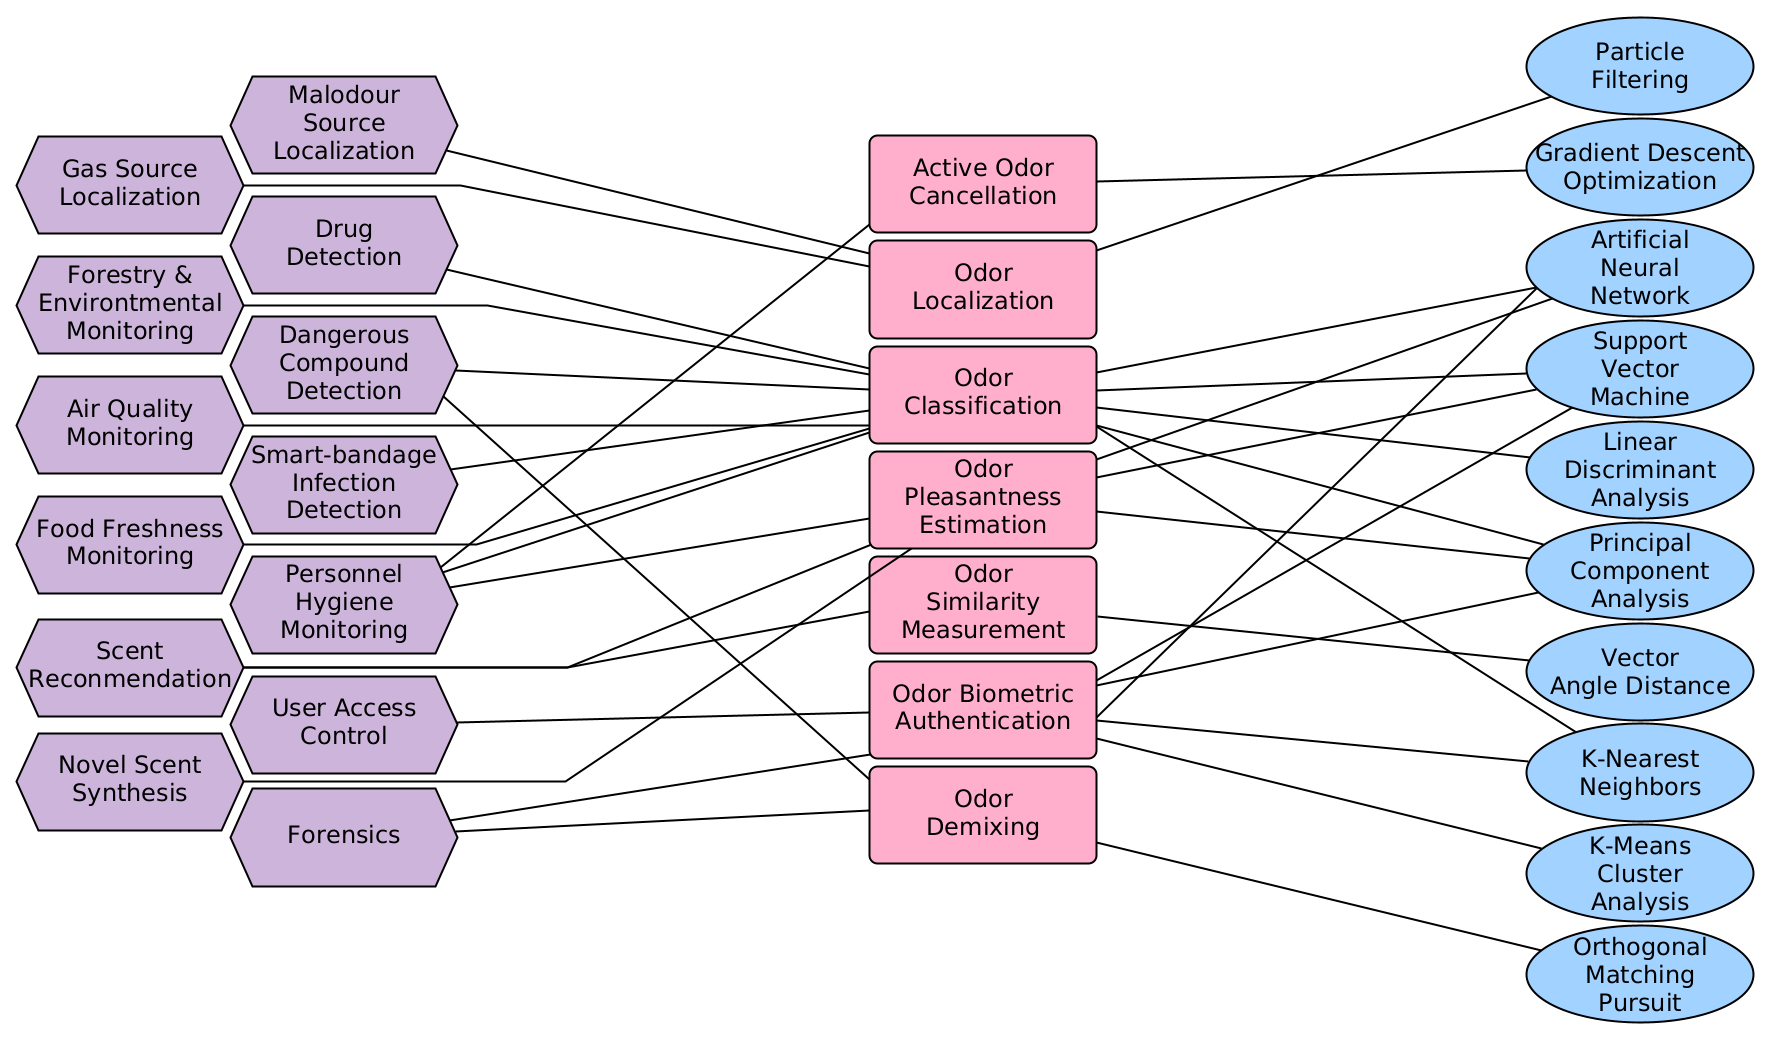
\includegraphics[width=\linewidth]{./figs/app_task_kernel.png}
    \caption{
        \small Graphical depiction of relationship between applications
        (\textcolor{purple}{hexagons}) which are composed from tasks
        (\textcolor{pink}{rectangles}).  Tasks are implemented using a
        computational kernel (\textcolor{blue}{ellipses}). Some tasks can be
        supported by multiple kernels.
    }
    \label{fig:app_task_kernel}
\end{wrapfigure}

In many
domains, the light computational requirements of \olfc{} algorithmic primitives
means the attention of architects is little needed. XR headsets, able to power
high resolution 3D graphics, for example, will have little trouble running
\olfc{} tasks.  However, there are domains with
extreme constraints which make \olfc{} interesting to architects.
Form factors such as wearables, (earrings, pendants, brooches, etc), bandages
(e.g., for detecting infections), adhesives (e.g., for body odor monitoring),
packaging (e.g., smart packages that detect food spoilage), swabs (for breath,
urine, body fluids-based diagnostics, for example), sensors-in-the-wild ( e.g.,
air quality monitoring, surface and ground water quality monitoring), etc., may
only allow for energy harvesting.  Field deployed sensors may need to maximize
limited battery energy capacities over long periods, or be self-powered.  In
these domains, both power and energy are stringent limitations.

 
%Fig.~\ref{fig:arch} presents an overview of \arch{}.
%\arch{}'s aim is to support energy efficient \olfc{}, given the
%lax performance requirements of \olfc{} applications, and the
%constrained energy budget available to edge devices.  Thus, \arch{} is designed
%for operating points at below nominal voltage.

\begin{wrapfigure}{r}{0.5\textwidth}
\centering
    
\includegraphics[width=\linewidth]{./figs/odor_arch.png}
    \caption{\small
            Organization of \arch{} as a \mcu{} with \vmacc{} and \cgra{}
            accelerators. Since \arch{} aims for energy efficiency, achieved by
            operating at low voltage and frequency, \arch{} exploits the lack
            of voltage scaling available to SRAMs to enable multiple SRAM
            accesses on a single port per clock cycle.
        }
    \label{fig:arch}
\end{wrapfigure}

Therefore, as a case study, we consider the architecture of a programmable
ultra-low-power \olfc{} hardware platform supporting low frequency
and voltage operation; programmability is supported to lower costs and to
maintain generality in a domain where applications are likely to evolve.  Our
architecture, \arch{} (Fig.~\ref{fig:arch}), is a heterogeneous reconfigurable
odor monitoring and analysis architecture consisting of a \SI{32}{\bit} RISC-V
MCU (RV32IM) with two integrated accelerators, both supporting fixed-point
operations. The \mcu{} is a four-stage, in order, scalar core based off of the
Open Hardware Group's CORE-V CV32 RISC-V IP~\cite{CV32_RISCV_IP}.  \arch{}
can be used to support \olfc{} systems, as in Fig.~\ref{fig:man_vs_machine}.

The first accelerator is a \SI{128}{\bit} packed SIMD unit which accelerates
fixed-point fused muliply accumulate operations on 4, 8, 16, and \SI{32}{\bit}
datatypes, to support the copious multiply-accumulates found in ANN, SVM,
LDA, PCA, VAD, and OMP algorithms.
Unlike a typical packed SIMD ISA extension, \arch{}'s \vmacc{} does not have an
additional SIMD register file.  Instead, data is accessed directly from memory,
which is made possible by the discrepancy between the core voltage at the
minimal energy operating points of \arch{} (Section~\ref{sec:results}), and the
SRAM's nominal voltage required to ensure memory retention. Additionally,
since the size of data memory required by many applications (Table~\ref{tab:kernels})
is small, the overhead of a dedicated SIMD register file may be large relative
to data memory in its entirety
(this is explored further in Section~\ref{sec:results}, where data memory is
replaced/augmented with a flip-flop based register file).

In order to exploit
data reuse found in linear algebraic workloads (i.e., mapping a sequence of
vectors by the same linear transformation), the \vmacc{} contains a buffer
which can be loaded with model parameters, or sensor data, neural network
activations, and other runtime data. The second accelerator is a coarse-grained
reconfigurable streaming dataflow architecture with nine heterogeneous PEs
(adder PEs, and multiply-accumulate PEs) arranged in a \(3\times 3\) grid, and
utilizing a bufferless, single-cycle, multi-hop routing network, as
in~\cite{wang2019hycube, gobieski2021snafu}. Each PE contains a small
(\SI{16}{\byte}) buffer, in which it can store model parameters, as well as
accumulated sums.  \arch{}'s \cgra{} is based off of the SNAFU low-power
reconfigurable architecture. PEs are capable of \SI{32}{\bit} width packed-SIMD
execution of multiplies and adds (i.e., $1\times$ \SI{32}{\bit} operation,
$2\times$ \SI{16}{\bit} operations, etc.).  The dataflows supported  on
the CGRA enables mapping convolution layers with various kernel sizes and strides.
This is important as although currently most \olfc{} ANNs are MLPs,
there do exist CNNs for \olfc{} applications, and the choice of the best
model for \olfc{} tasks is still being litigated.

Both accelerators support efficient packed SIMD addition and multiplication for
datatypes of varying width, as wide adders and multipliers can be
recursively built from narrow adders and multipliers.
Wide adders are built from narrow adders via carry-out propagation.
Wide multipliers are built from narrow multipliers via convolution
(or, polynomial multiplication), as in Fig.~\ref{fig:poly_mul}.
This figure shows how narrow multipliers can be used to compute partial
products for a wider multiplier (Fig.~\ref{fig:poly_mul_pp}).
These partial products are then summed
to generate wider multiplier's product (Fig.~\ref{fig:poly_mul_red}).
When configured to support the `narrow' datatype, the multiplier simply
outputs the \(A_1B_1\) and \(A_0B_0\) products, while when configured
to support the `wide' datatype, the multiplier outputs the full \(AB\)
product.  This technique can be recursively applied, which enables
\SI{8}{\bit}, \SI{16}{\bit}, and \SI{32}{\bit} multipliers to all be built
from \SI{4}{\bit} multiplier primitives.
Note that when operating on the `narrow` datatype, there are twice as many
partial product generating multipliers as required.  These multipliers can
be clock-gated, reducing dynamic power consumption in the multipliers and
the adder reduction tree.  A second use for these multipliers could be to increase
the total width of the packed SIMD units. However, doing so would require
doubling the data memory bandwidth.  At ultra-low frequency operating points,
this may be possible, however, it is not explored in \arch{}.
In fixed-point arithmetic, shifters are used to rescale products.
These are implemented for the different datatypes in parallel, and the output
is muxed based on the datatype required. In both the \vmacc{} and the \cgra{}
PEs, the multipliers are pipelined to ensure they meet timing at nominal
voltage and frequency.  Exact location of pipeline registers is determined by
register retiming.
To support ANNs, both accelerators are programmed to perform either linear or
reLU activations on accumulated data before writing the results to data memory.

\begin{wrapfigure}{l}{0.5\linewidth}
\centering
\begin{subfigure}{\linewidth}
    
\includegraphics[width=\linewidth]{./figs/poly_mul.png}
    \caption{Partial product computation.}
    \label{fig:poly_mul_pp}
\end{subfigure}

\begin{subfigure}{\linewidth}
    
\includegraphics[width=\linewidth]{./figs/poly_mul_reduction.png}
    \caption{Partial product reduction.}
    \label{fig:poly_mul_red}
\end{subfigure}
\caption{Narrow multipliers are converted into wider multipliers via
convolution, or polynomial multiplication.}
\label{fig:poly_mul}
\end{wrapfigure}

The accelerators are given direct access to data memory, which enables the
\mcu{} to be idle while the accelerators work.  The accelerators signal
completion of their work via IRQ lines.  The core can also choose to poll the
accelerator's status register if the accelerator is expected to finish its task
quickly.  Since accelerator launch costs are small (due to the small size of
the CGRA, and small number of operations supported by both architectures), and
the often large number of linear operations between non-linear operations
(Table~\ref{tab:kernels}), the accelerators are focused on accelerating linear
operations, and specifically fused multiply-accumulates.  This means that
non-linear operations are left for execution on the \mcu{}.

\arch{}  uses a modified Harvard architecture, in which program instructions
and model parameters are stored in a non-volatile ROM, while read-write data
is stored in an SRAM-based data memory.  Since standard SRAMs cannot be safely
voltage scaled without error detection and correction coding~\cite{kumar2009sram}, a single
SRAM bank may be accessed multiple times by the DMA controller in each compute
clock cycle.

\arch{} may be run in one of three modes.  In MCU mode, only the \mcu{} is
active, with both accelerators powered off. In MCU+SIMD mode, the \mcu{} and
\vmacc{} are used, but the \cgra{} is powered off.  In MCU+CGRA mode, the
\mcu{} and \cgra{} are powered, while the \vmacc{} is powered off. Which mode
to use in deployment is determined statically by the programmer after analyzing
performance in the different modes.

\begin{figure*}[h]
    \centering
    \begin{subfigure}{0.3\textwidth}
        \centering
        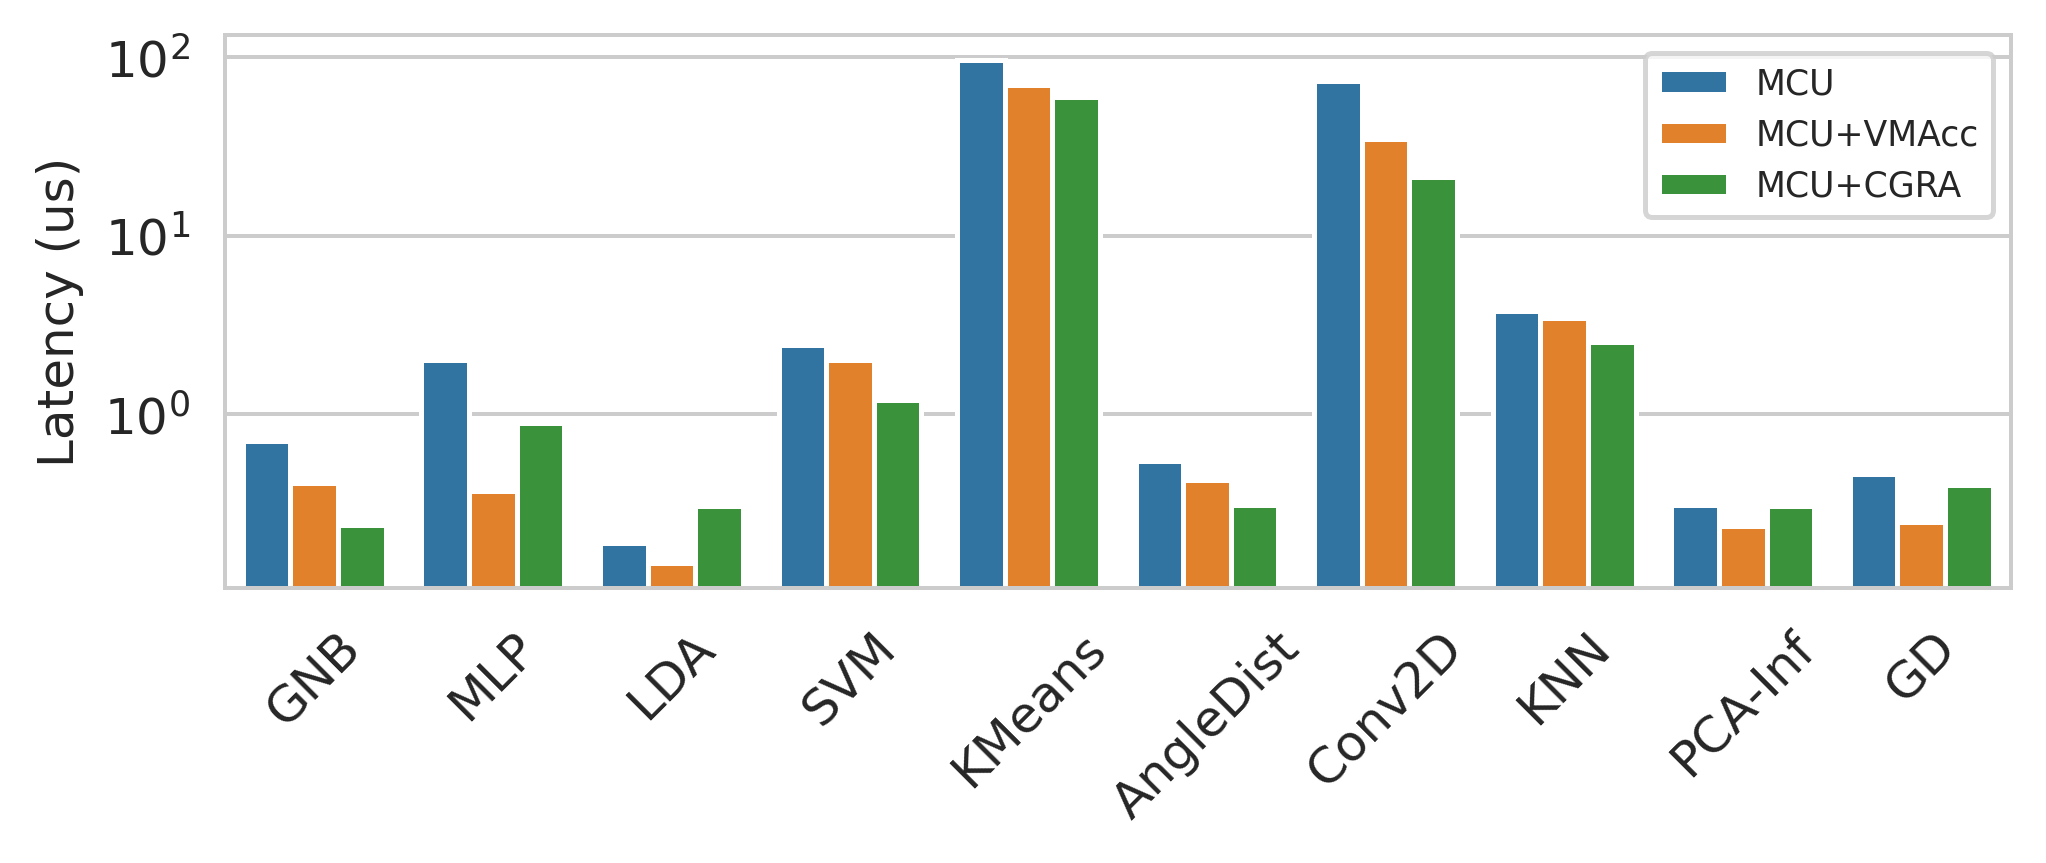
\includegraphics[width=1.0\linewidth]
            {./figs/one_volt_latency.png}
        \caption{\small Performance of \arch{}'s modes across benchmarks.}
        \label{fig:baseline_latency}
    \end{subfigure}
    \begin{subfigure}{0.3\textwidth}
        \centering
        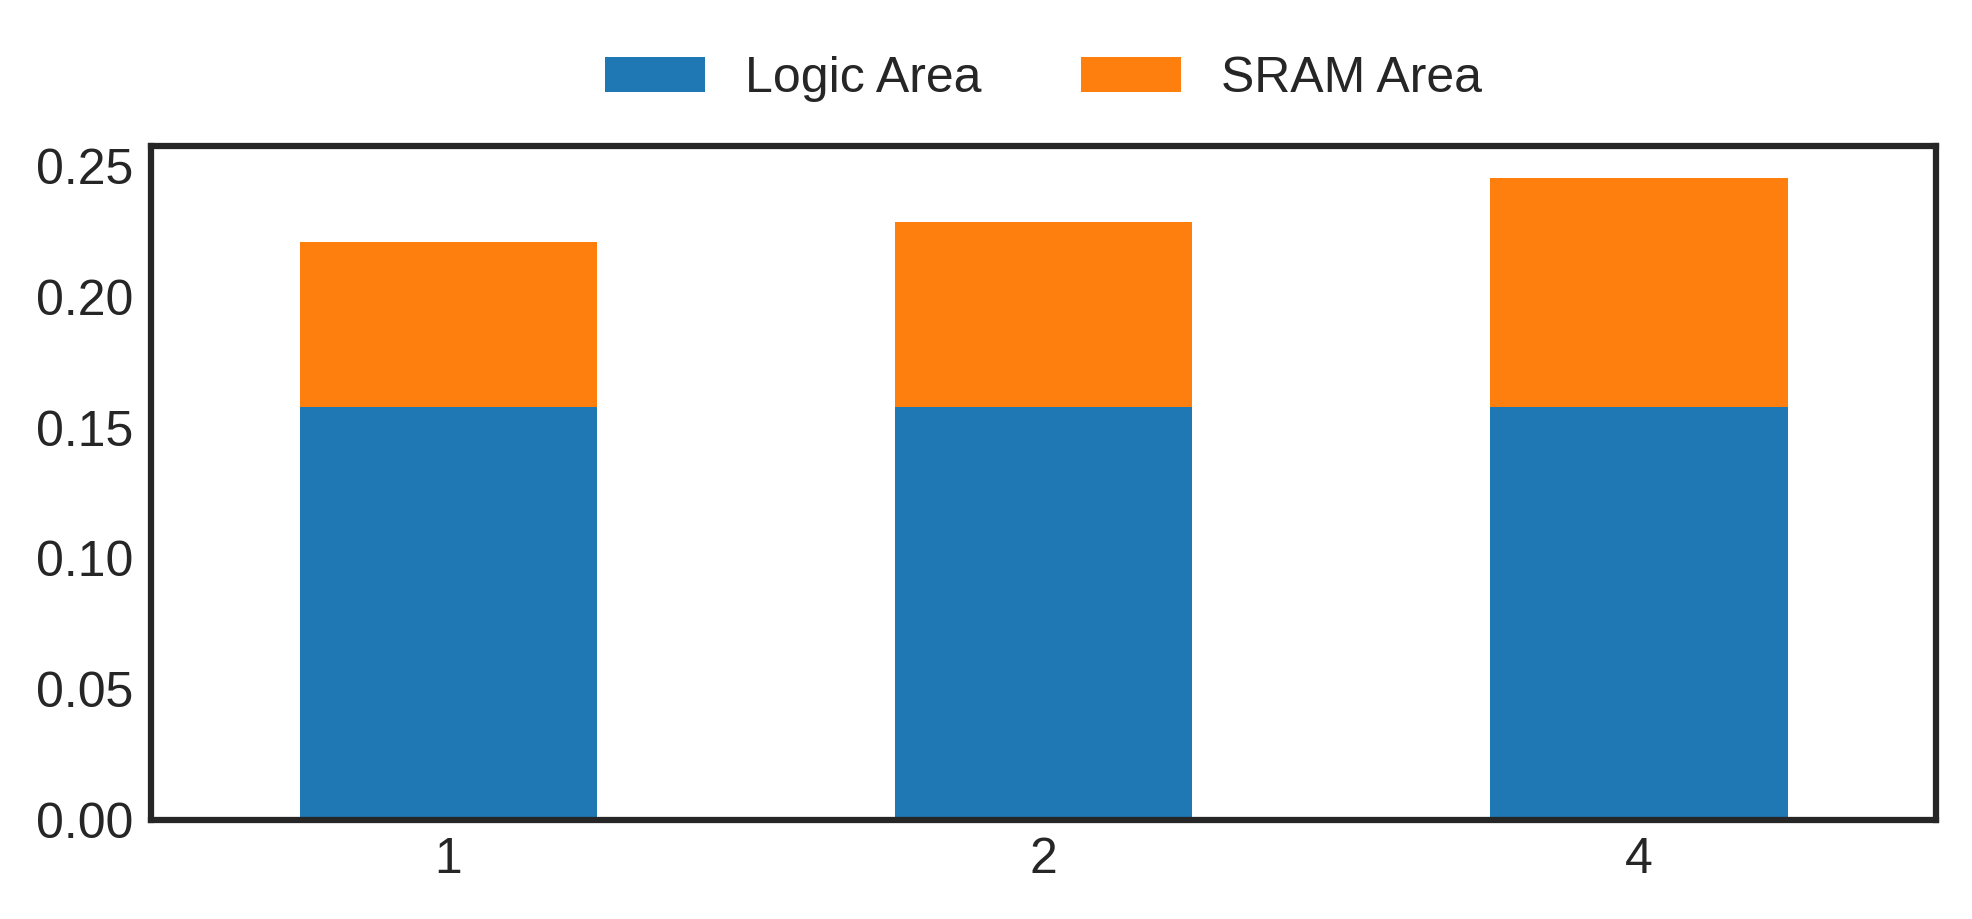
\includegraphics[width=1.0\linewidth]
            {./figs/one_volt_area.png}
        \caption{\small Area needed to support \arch{}'s modes with
            SRAM organized into one, two, and four banks.
        }
        \label{fig:baseline_area}
    \end{subfigure}
    \begin{subfigure}{0.3\textwidth}
        \centering
        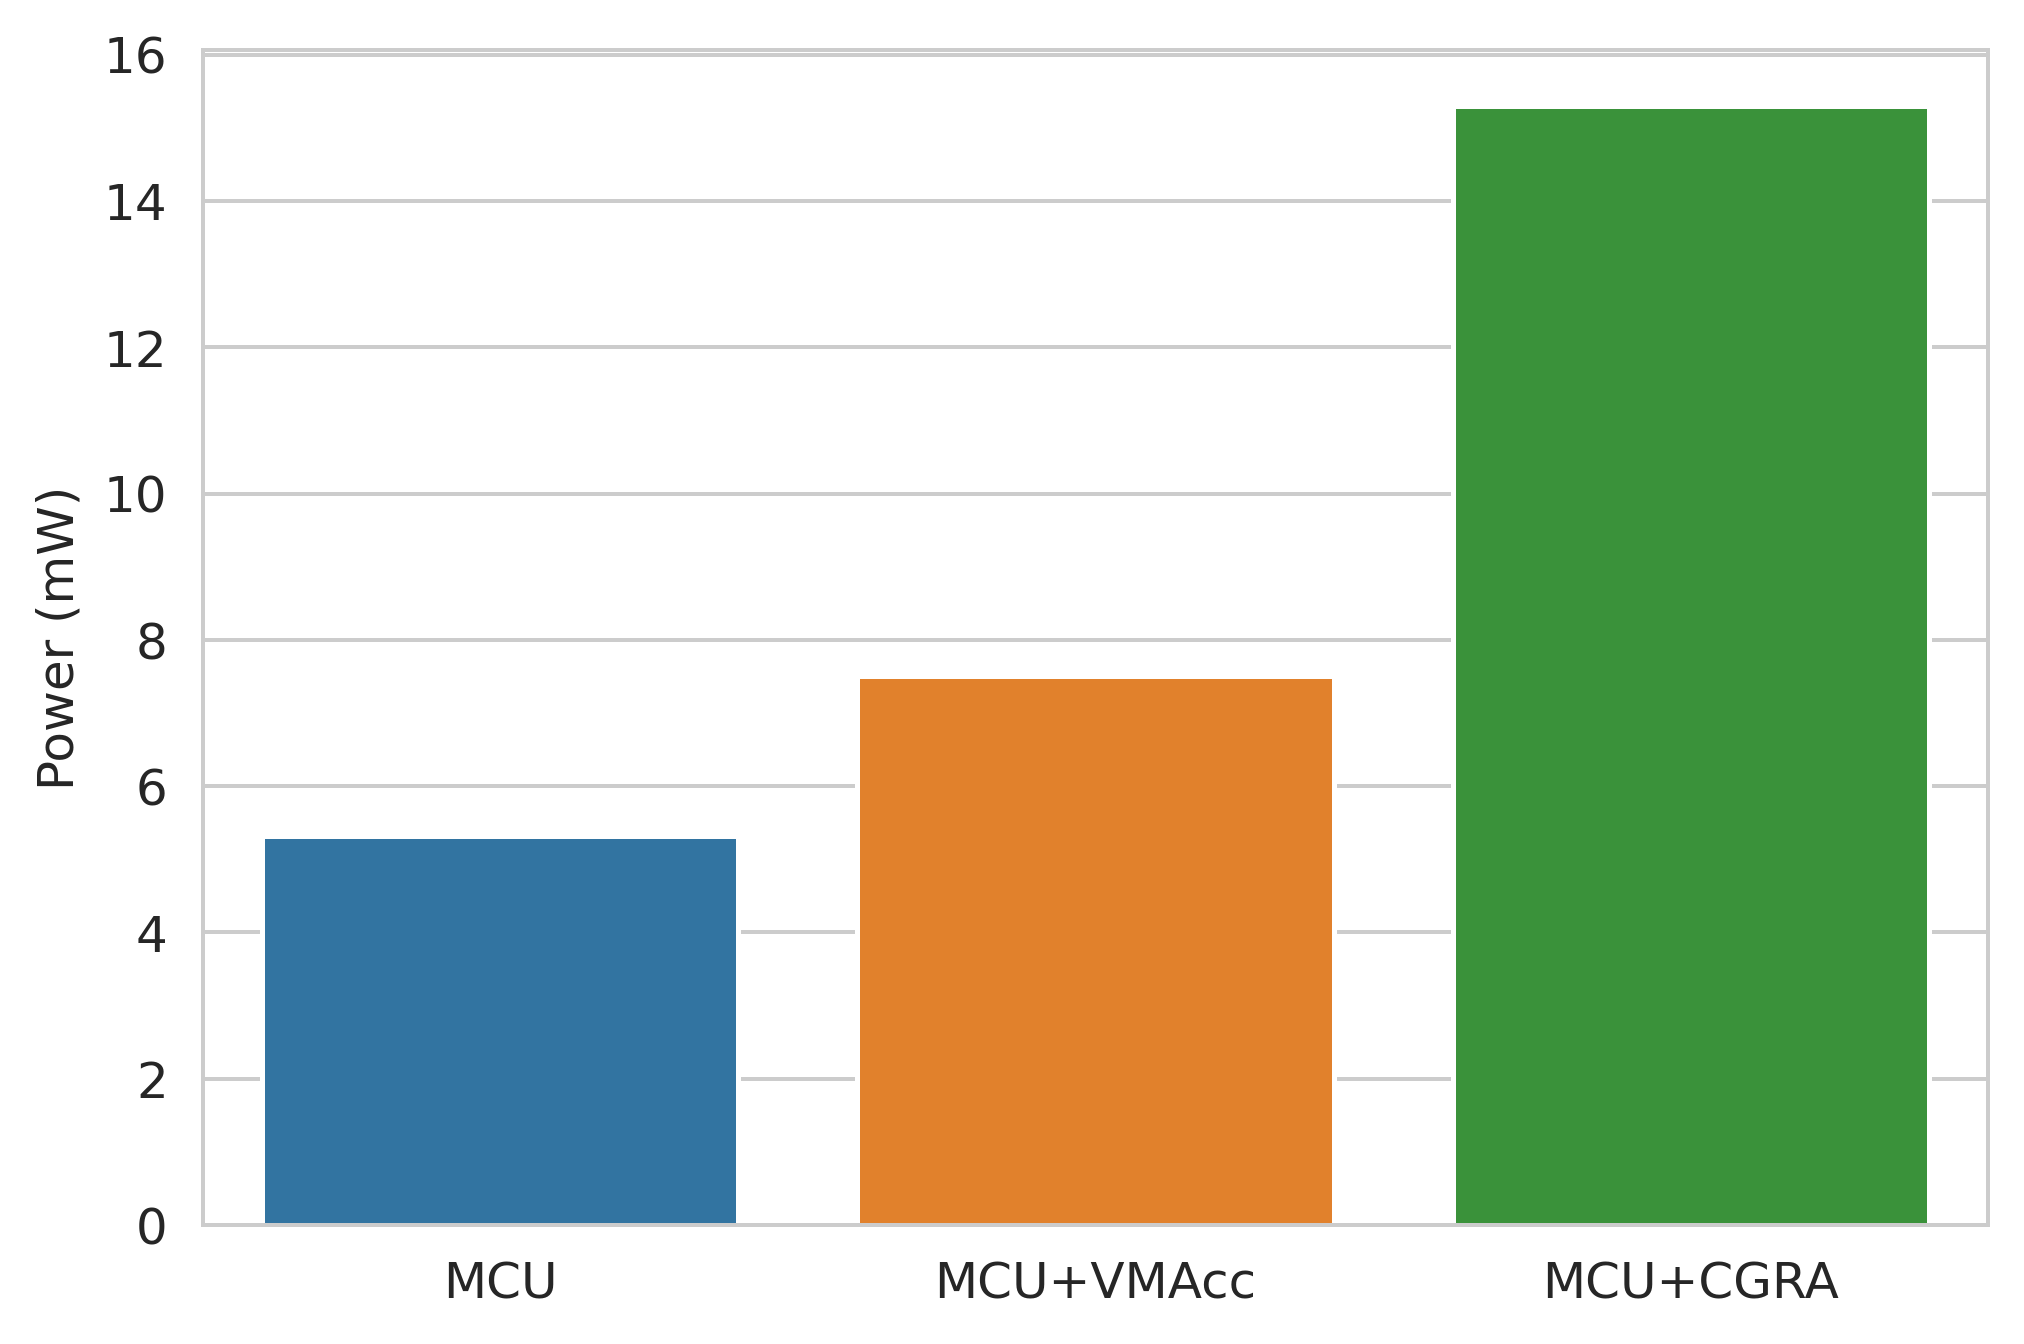
\includegraphics[width=1.0\linewidth]
            {./figs/one_volt_power.png}
        \caption{\small Power consumption of \arch{}'s modes.}
        \label{fig:baseline_power}
    \end{subfigure}
    \\
    \begin{subfigure}{\linewidth}
        \centering
        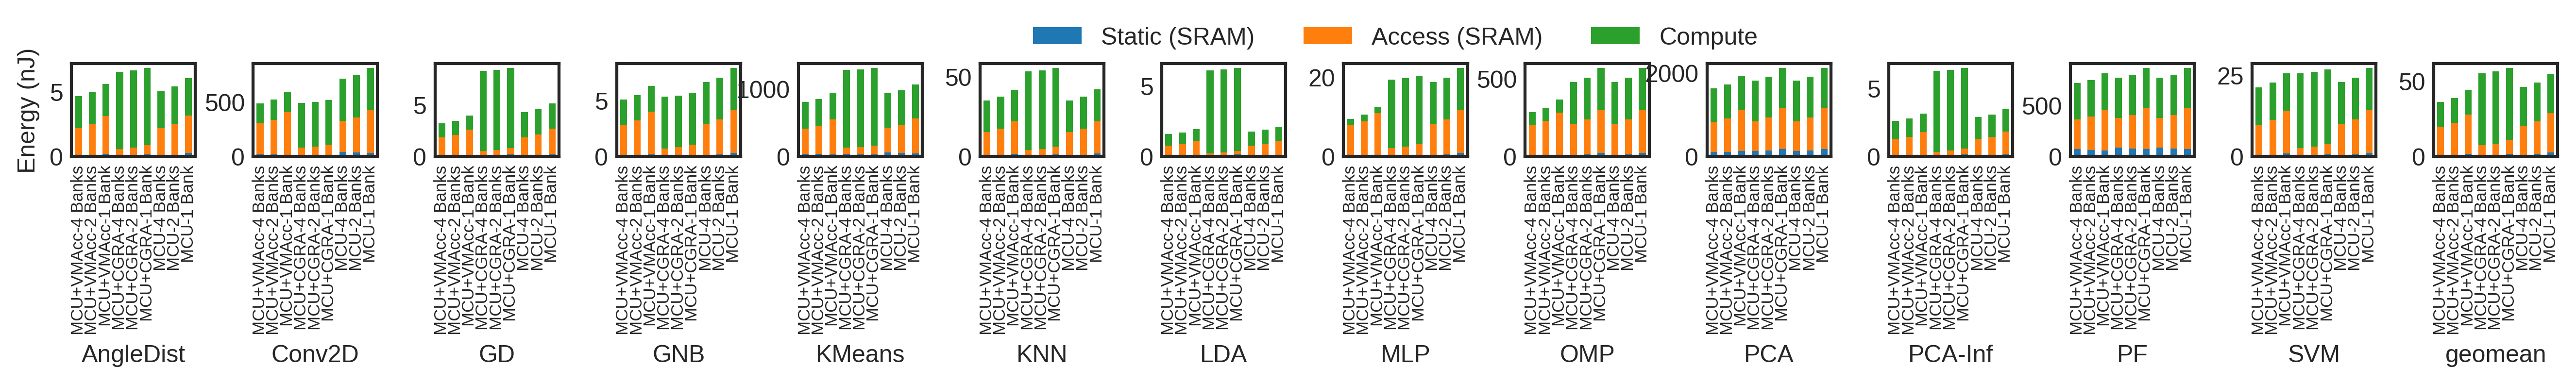
\includegraphics[width=1.0\linewidth, height=0.25\textwidth]
            {./figs/one_volt_total_energy.png}
        \caption{\small Total energy consumption of \arch{}'s modes
        for each kernel and with several SRAM organizations.}
        \label{fig:baseline_energy}
    \end{subfigure}
    \caption{\small Baseline Results.}
    \label{fig:baseline_results}
\end{figure*}


Fig.~\ref{fig:baseline_results} shows baseline results for \arch{} with several
SRAM organizations at nominal frequency (\SI{600}{\mega\hertz}) and voltage
(\SI{1}{\volt}). \arch{}'s performance on the kernels is shown in
Fig.~\ref{fig:baseline_latency}, broken down by \arch{} mode of operation.
Across all kernels, the mode with the \vmacc{} consistently outperform
the \mcu{} baseline (Fig.~\ref{fig:baseline_latency}). Similarly, for most
kernels, the \cgra{} based mode outperforms the \mcu{} baseline.
However, for applications with very small amounts of compute (e.g., LDA), the
CGRA configuration and launch overhead offset the speed-up provided by the
CGRA, resulting in faster execution on the \mcu{} alone. Despite this, the CGRA
is the best performer on a number of benchmarks, including Conv2D - a kernel
vital in CNNs, and SVM. The high performance of the parallel architectures is
due to the prevalence of multiply-accumulates within the kernels, as discussed
in Section~\ref{sec:workloads}.

The same pattern also emerges for energy (Fig.~\ref{fig:baseline_energy}), with
mode with the MCU+SIMD outperforming the MCU alone in energy efficiency, while
the MCU+CGRA only outperforms the MCU on several kernels and outperform the
MCU+SIMD on Conv2D, due to the high power consumption of the MCU+CGRA. The
figure also shows the importance of using multiple SRAM banks. By dividing the
SRAM into banks, banks which are unneeded for a given application kernel may be
put into retention mode, eliminating nearly all power consumption of the SRAM.

Fig.~\ref{fig:high_power_energy_banking} shows the absolute energy consumed by
\arch{}'s modes at their minimal energy operating point (MEOP) on a
\SI{10}{\milli\watt} nominal power budget.  The MEOPs are \SI{0.4}{\volt} and
\SI{357}{\mega\hertz} for the MCU and and MCU+SIMD, and \SI{0.4}{\volt} and
\SI{119}{\mega\hertz} for the MCU+CGRA. Operating at the MEOP provides
significant energy efficiency improvement over the nominal operating point due
to reduction in dynamic power which decreases superlinearly with reduction in
frequency. This can be seen by the growth in the proportion of energy consumed
by SRAM reads and writes, relative to Fig.~\ref{fig:baseline_energy}. Operating
at MEOP enables the MCU+CGRA to become the most energy efficient mode on most
kernels, with MCU+SIMD being the most energy efficient on OMP and PF. On
average, the MEOP provides \MeopImprovementMcu{}, \MeopImprovementVMAcc{}, and
\(\MeopImprovementCgra{}\times\) improvement over the nominal operating points
for the \mcu{}, \mcu{}+\vmacc{}, and \mcu{}+\cgra{} modes, respectively.

\begin{figure*}[tb]
    \centering
    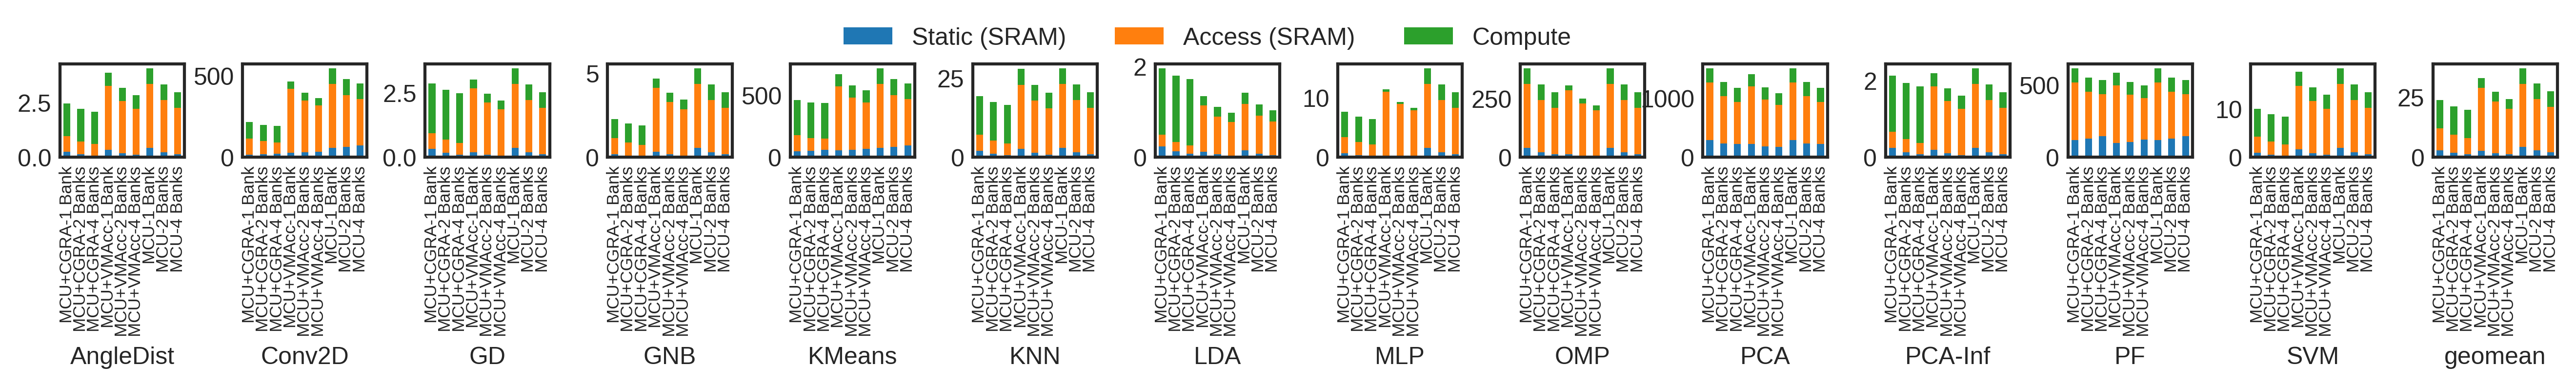
\includegraphics[width=1.0\linewidth]{./figs/high_power_energy_banking.png}
    \caption{\small
        Energy consumption at the MEOP on each kernel with different SRAM
        organizations: One 2048 word SRAM, two 1024 word SRAMs, and four 512
        word SRAMs.
    }
    \label{fig:high_power_energy_banking}
\end{figure*}

% \input{./tables/mass-data.tex}
% Table~\ref{tab:mass-data} contains details of energy breakdowns for each
% kernel in each \arch{} mode for several SRAM organizations at the minimal
% energy operating point.

\begin{wrapfigure}{l}{0.5\linewidth}
    \centering
    \begin{subfigure}{\linewidth}
        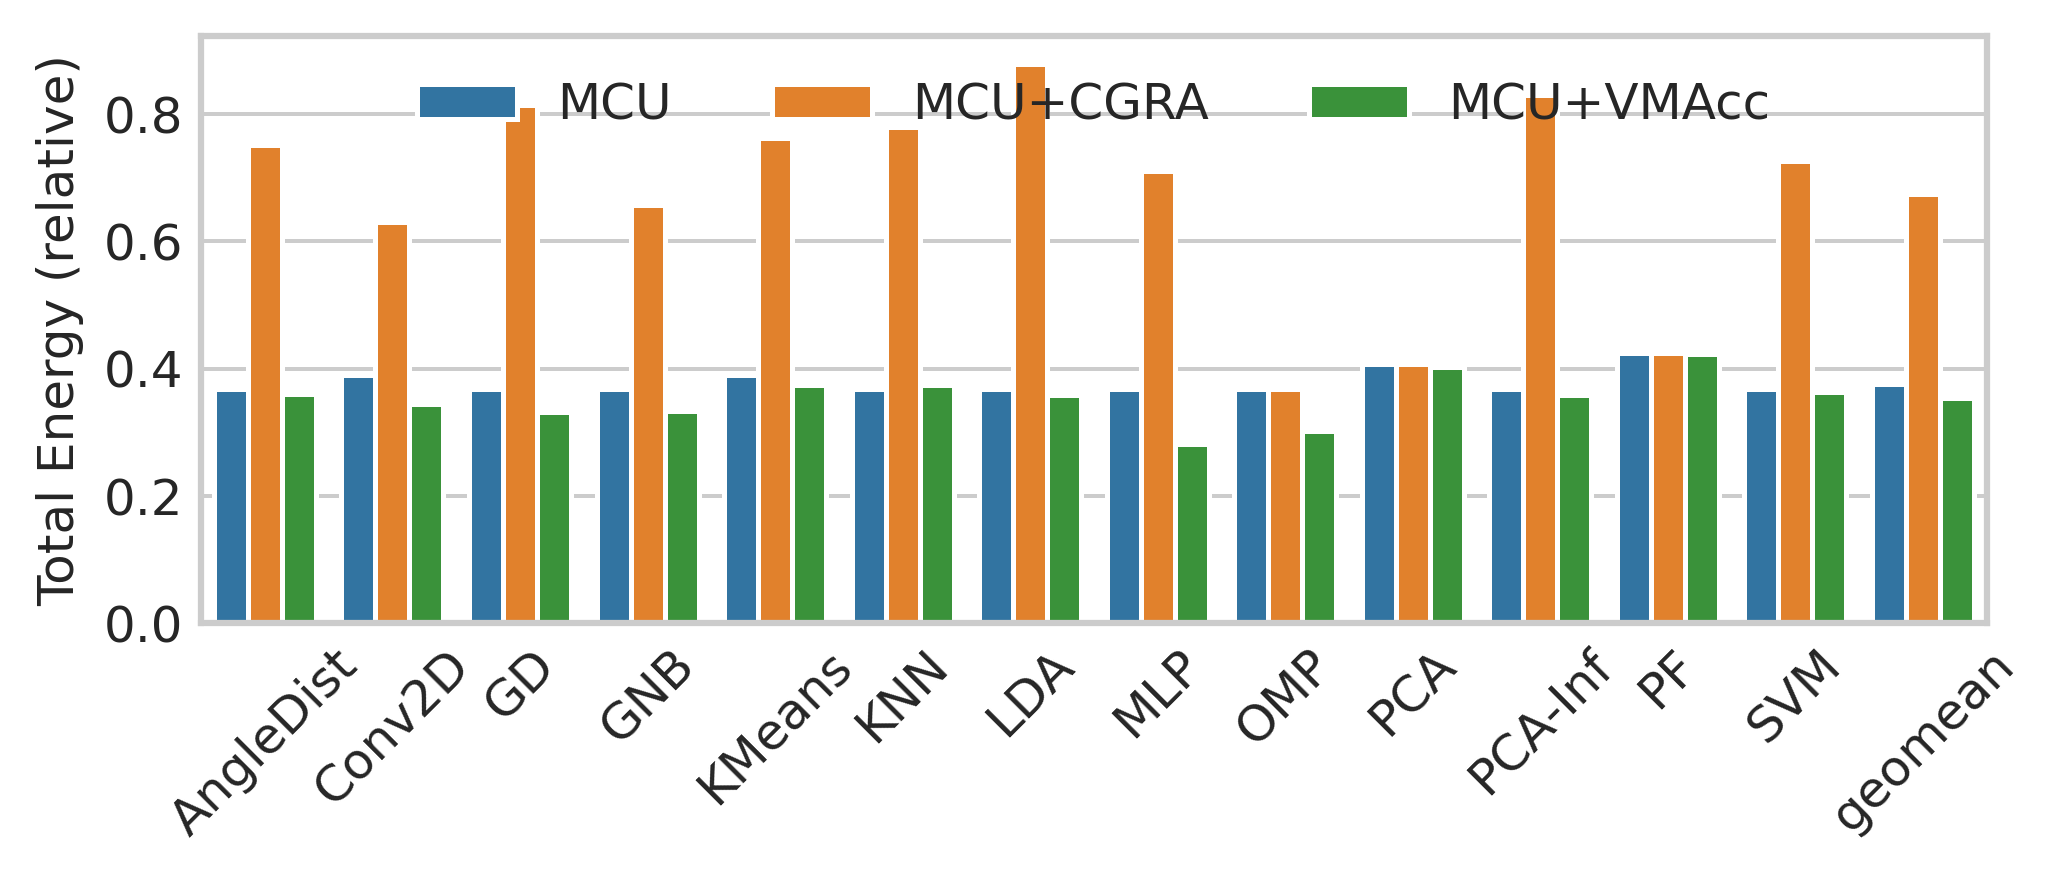
\includegraphics[width=1.0\linewidth]
            {./figs/4KB_tech.png}
        \caption{
            \small Energy achieved at MEOP for \arch{}'s modes across kernels
            with \SI{4}{\kibi\byte} memories built out of flip-flops relative
            to execution with a standard \SI{4}{\kibi\byte} SRAM.
        }
        \label{fig:four_kb_tech}
    \end{subfigure}

    \begin{subfigure}{\linewidth}
        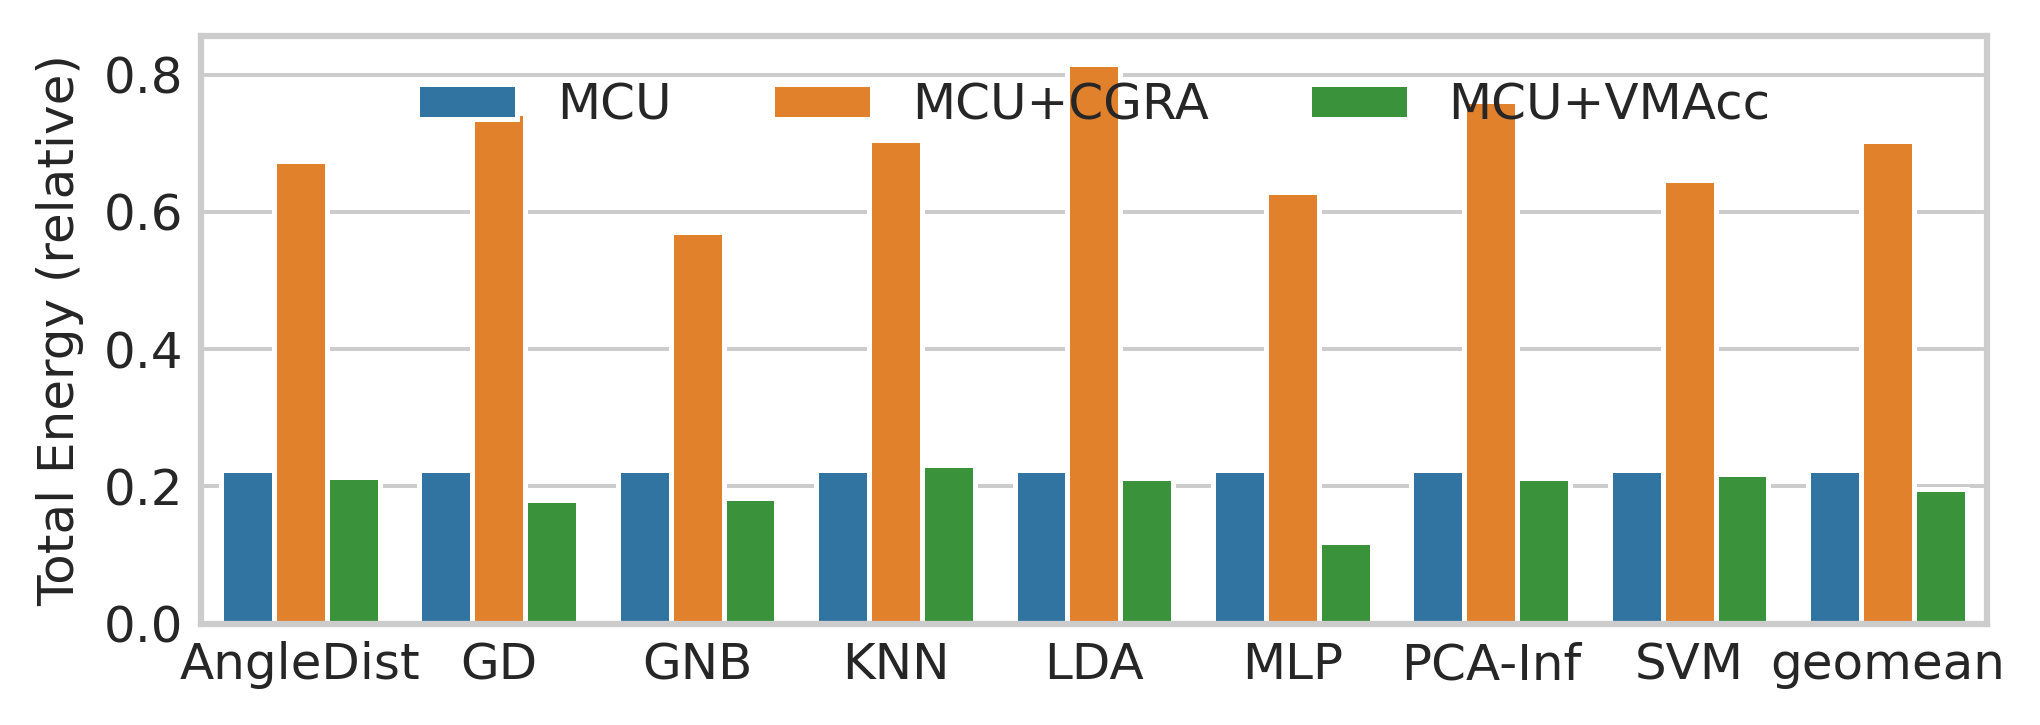
\includegraphics[width=1.0\linewidth]
            {./figs/scratchpad_energy.png}
        \caption{
            \small Energy achieved at MEOP for \arch{}'s modes across kernels
            with a 64-word memory built out of flip-flops relative to
            execution with a standard \SI{4}{\kibi\byte} SRAM.
        }
        \label{fig:scratch_tech}
    \end{subfigure}
    \caption{Replacing SRAMs with flip-flops has a dramatic effect on
    total energy consumption for some of \arch{}'s modes of operation.}
    \label{fig:sram_ff}
\end{wrapfigure}

Fig.~\ref{fig:sram_ff} shows the effects of replacing SRAM with 
memories built out of flip-flops.
In Fig.~\ref{fig:four_kb_tech}, the entire \SI{4}{\kibi\byte} SRAM is replaced
by an equivalently sized memory built from flip-flops.  This enables voltage
scaling to be applied to the memory, whereas with a standard 6T-SRAM, scaling
voltage down to the core's MEOP would likely result in data corruption. The
effects of this are very positive for the MCU and MCU+SIMD modes, both
seeing an over 60\% decrease in energy consumption. In
these modes, SRAM access energy dominates energy consumption.  Thus, the lower
energy of the flip-flop accesses leads to significant energy efficiency
improvements.  This comes despite the fact that the voltage-scaled memory
inhibits the MCU+SIMD from operating at full throughput, due to voltage scaling
of the flip-flop memory leading to increased access latencies. This fact also
mitigates the effectiveness of this technique in the MCU+CGRA mode.
Also, in this mode, compute energy, rather than memory access energy, is the
predominant energy consumption.

In Fig.~\ref{fig:scratch_tech}, \arch{}'s memory is replaced by a small
\SI{256}{\byte} flip-flop based memory.  For kernels with limited data memory
requirements (which is the majority of the studied kernels), this memory
organization results in significant (\(> 4\times\)) energy savings in MCU
and MCU+SIMD modes.  Here, once again, the MCU+CGRA mode sees
less improvement in energy consumption due to increased execution latency, and a
smaller proportion of energy consumption being due to SRAM accesses in
the baseline.  Since the small memory consumes far less dynamic and static
power than the \SI{4}{\kibi\byte} memory, the improvement over the baseline
grows, with the MCU+SIMD mode reducing power by over 80\%.
The smaller memory also helps MCU+CGRA mode, which sees a 30\% reduction
in energy consumption.
Across all kernels, this data memory
organization lead to additional \FFImprovementMcu{}, \FFImprovementVMAcc{}, and
\(\FFImprovementCgra{}\times\) improvements in energy efficiency on average.

The energy savings from flip-flop based memories come at a significant area
cost. The area of \arch{} with \SI{4}{\kibi\byte} memory is
\SI{0.53}{\milli\meter\squared}, a 193\% increase over \arch{} with an equally
sized SRAM.
The overhead of adding the \SI{256}{\byte} memory to \arch{}, however, is small.
Using the small memory as a scratchpad, while retaining the standard SRAM
for applications which may require more memory, results in an area increase
of only 10.3\%.
This demonstrates that, in the the low-power \olfc{} domain, the small memory
requirements of algorithms has a major impact on choice of computer
architecture, with significant trade-offs between area (and hence cost)
and energy efficiency.  This trade-off can be mittigated by using hybrid
memories, composed of small capacity, low density, low power memories, and
larger, denser, higher power memories.


\begin{figure}[h]
    \centering
    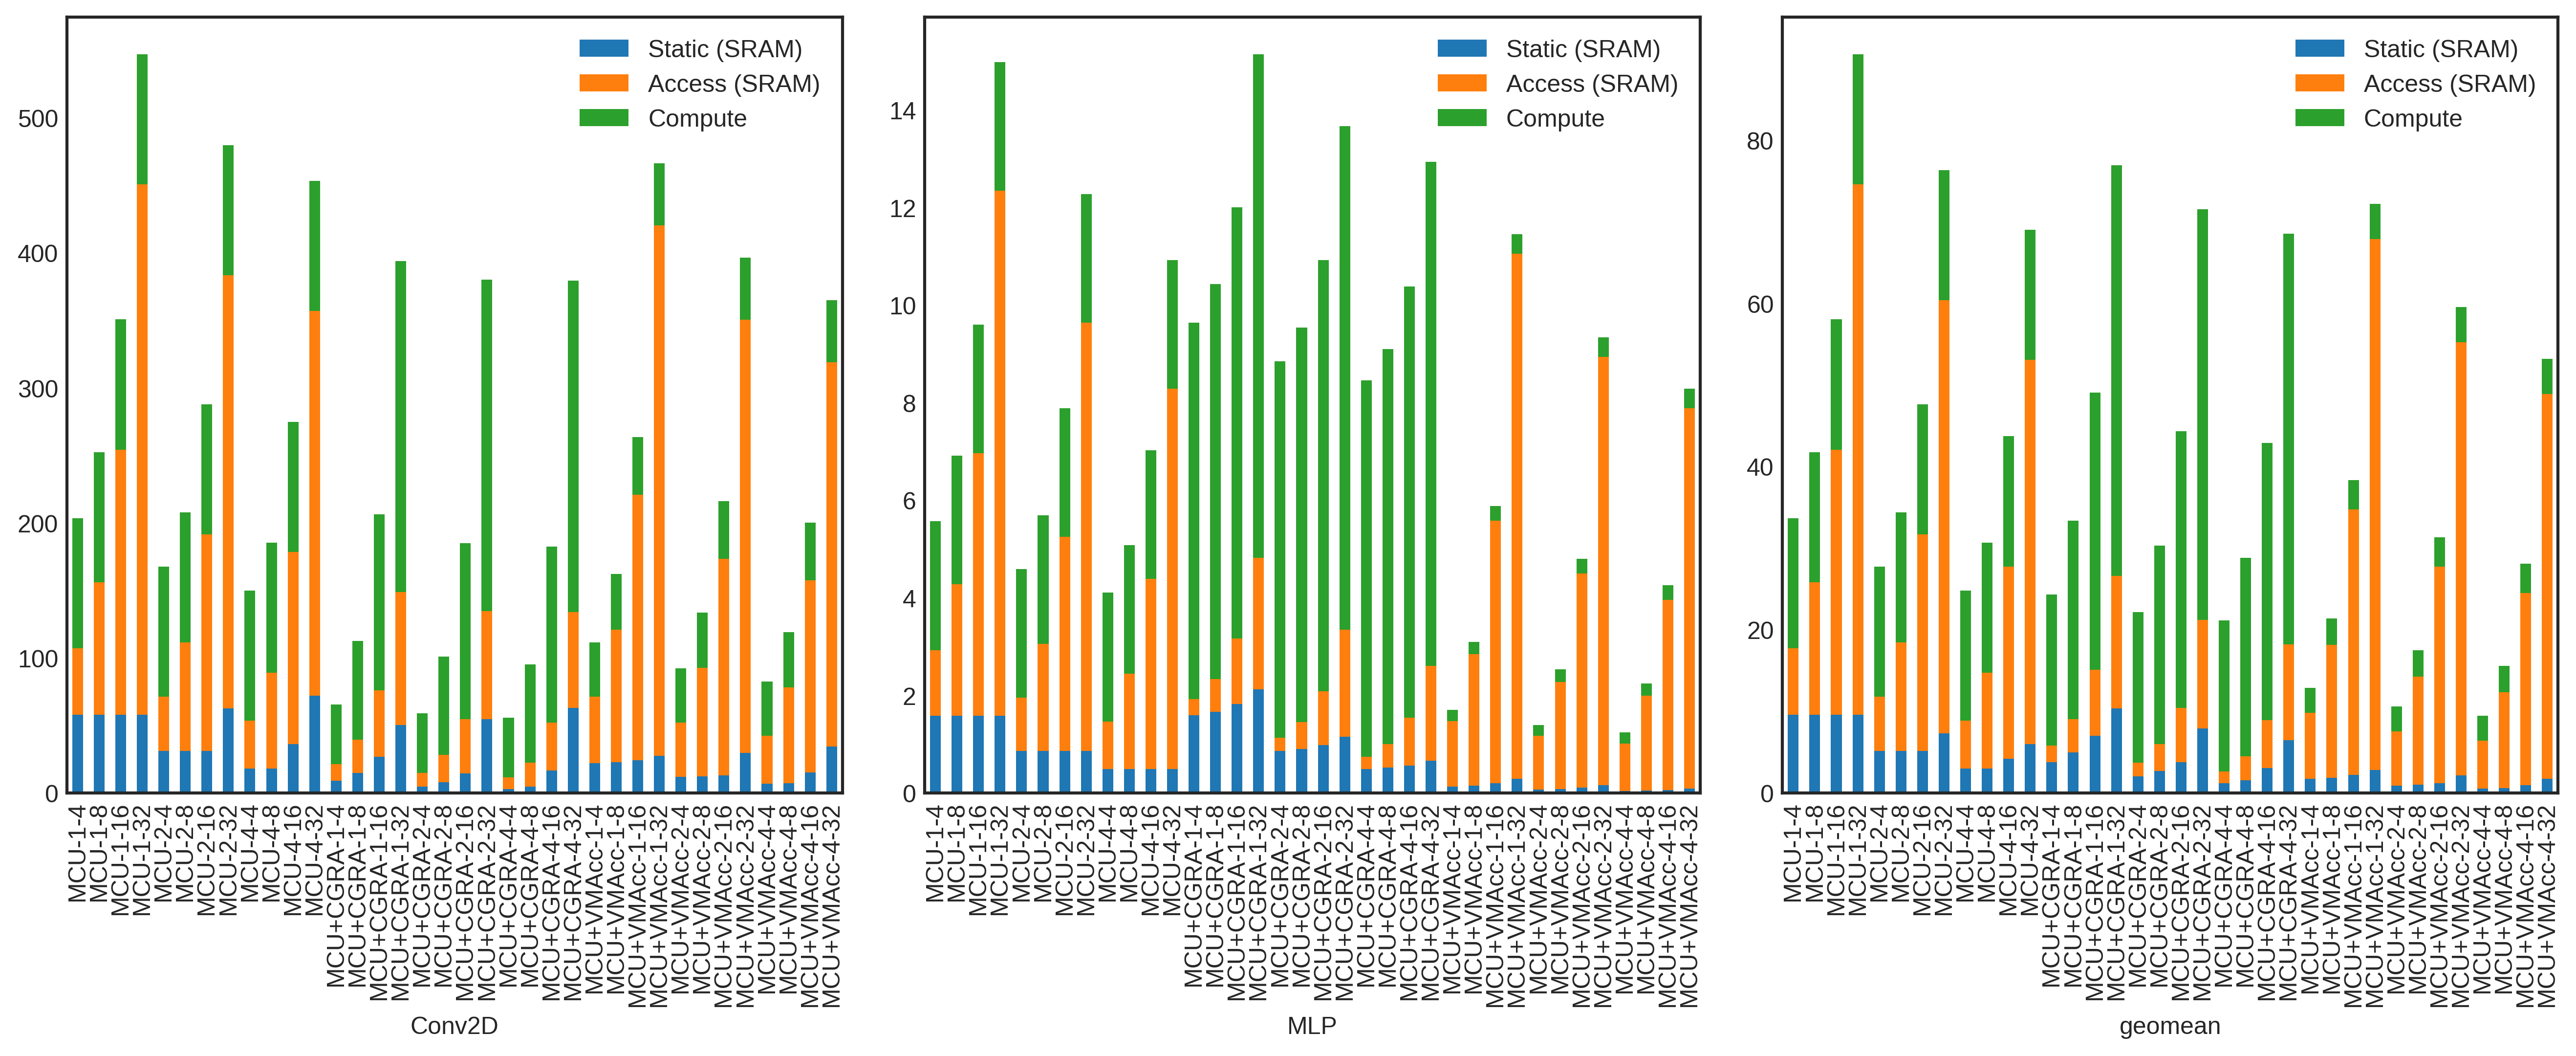
\includegraphics[width=1.0\linewidth]{./figs/high_power_energy_banking_quant.png}
    \caption{\small
        Data quantization leads to decreased energy for appropriate
        kernels.  Further, data quantization's benefits are orthogonal
        to benefits from banking.
    }
    \label{fig:banking_quant}
\end{figure}

%A large corpus of work has demonstrated that the data precision used to encode
%neural network parameters \textit{and} activations can be reduced with
%little impact on classification accuracy~\cite{}.  As such, 
We also evaluate how
parameter and activation quantization impacts energy efficiency in
\olfc{} using the two ANN related kernels (MLP and Conv2D).
Figure~\ref{fig:banking_quant} shows the effects of data quantization
on the architectures at MEOP for a variety of different SRAM organizations.
Benefits for the \mcu{} are the most limited, as the \mcu{} only takes advantage
of quantization through reduction in number of memory accesses.
The \cgra{} and \vmacc{} also see benefit from reduced latency, as they are able to
decrease the latency of the acceleratable portion of the computation via packed
SIMD execution. Packed SIMD execution on multiplies and adds, as is needed
by the \vmacc{} and \cgra{} for the MLP and Conv2D workloads, has negligible
hardware overhead, as word-length multipliers and adders can be built by
recursively composing half-word, byte, and nibble length multipliers
(via convolution) and adders (via carry propagation).
Although not evaluated, the \cgra{} and \vmacc{} could also see decreased
dynamic energy consumption via input gating, as logic used to transform
narrow (e.g., \SI{4}{\bit}) multiplications into wide (e.g., \SI{32}{\bit})
multiplications is not needed when performing quantized operations.
Fig.~\ref{fig:banking_quant} also shows that the improvements from quantization
and from banking are sufficiently orthogonal of one another that 
they can be deployed simultaneously to achieve the effects of both without
interference.

Indeed, there is also a \textit{synergistic} relationship between
banking and quantization, which can be most clearly seen in the Conv2D results
for the \mcu{} mode. In this mode, since performance is independent of both
banking and quantization, when the SRAM bank is available, the amount of
SRAM leakage energy is fixed and independent of quantization.
However, when two banks are used, since quantiztion leads to a decrease
in the total amount of memory required to execute the Conv2D kernel, a single 
SRAM bank may be placed in retention for 4, 8, and \SI{16}{\bit} data, while
both SRAM banks must be active for \SI{32}{\bit} data.  The granularity
of this again increases when four banks are available, with 4 and \SI{8}{\bit}
data types only needing a single bank, while \SI{16}{\bit} data requires
two banks, and \SI{32}{\bit} data requires all four banks.
This same phenomenon plays out with the other modes. However, SRAM leakage
energy in these cases is also impacted by quantization's impact on performance.

\arch{}'s results provide several interesting insights into \olfc{}.
First, when area is not a concern (consider compute area on the back-side of
a solar harvester), a programmable heterogeneous architecture will outperform
monolithic architectures and should be used.  Second, parallel SIMD and dataflow
architectures are effective at improving energy efficiency of even the
very small \olfc{} workloads --- this is not self-evident, as many \olfc{} workloads
have orders of magnitude less compute than even traditional sensor processing.
Third, memory organization has a major impact on energy efficiency in \olfc{},
due to the wide ranging amounts of data memory required by its workloads.


Figure~\ref{fig:vs_baselines} shows how a heterogeneous architecture such as
\arch{} outperforms an an ULP MCU, an ULP MCU with a ULP SIMD unit, and a ULP
CGRA (the individual operating modes of \arch{}, respectively) by
\BaselineGeomeanMcu{}, \BaselineGeomeanVmacc{}, and
\BaselineGeomeanCgra{}$\times$ on average in energy efficiency (in terms of
energy at MEOP). This demonstrates the benefit of our architecture against
possible alternatives.

\begin{wrapfigure}{l}{0.5\linewidth}
\centering
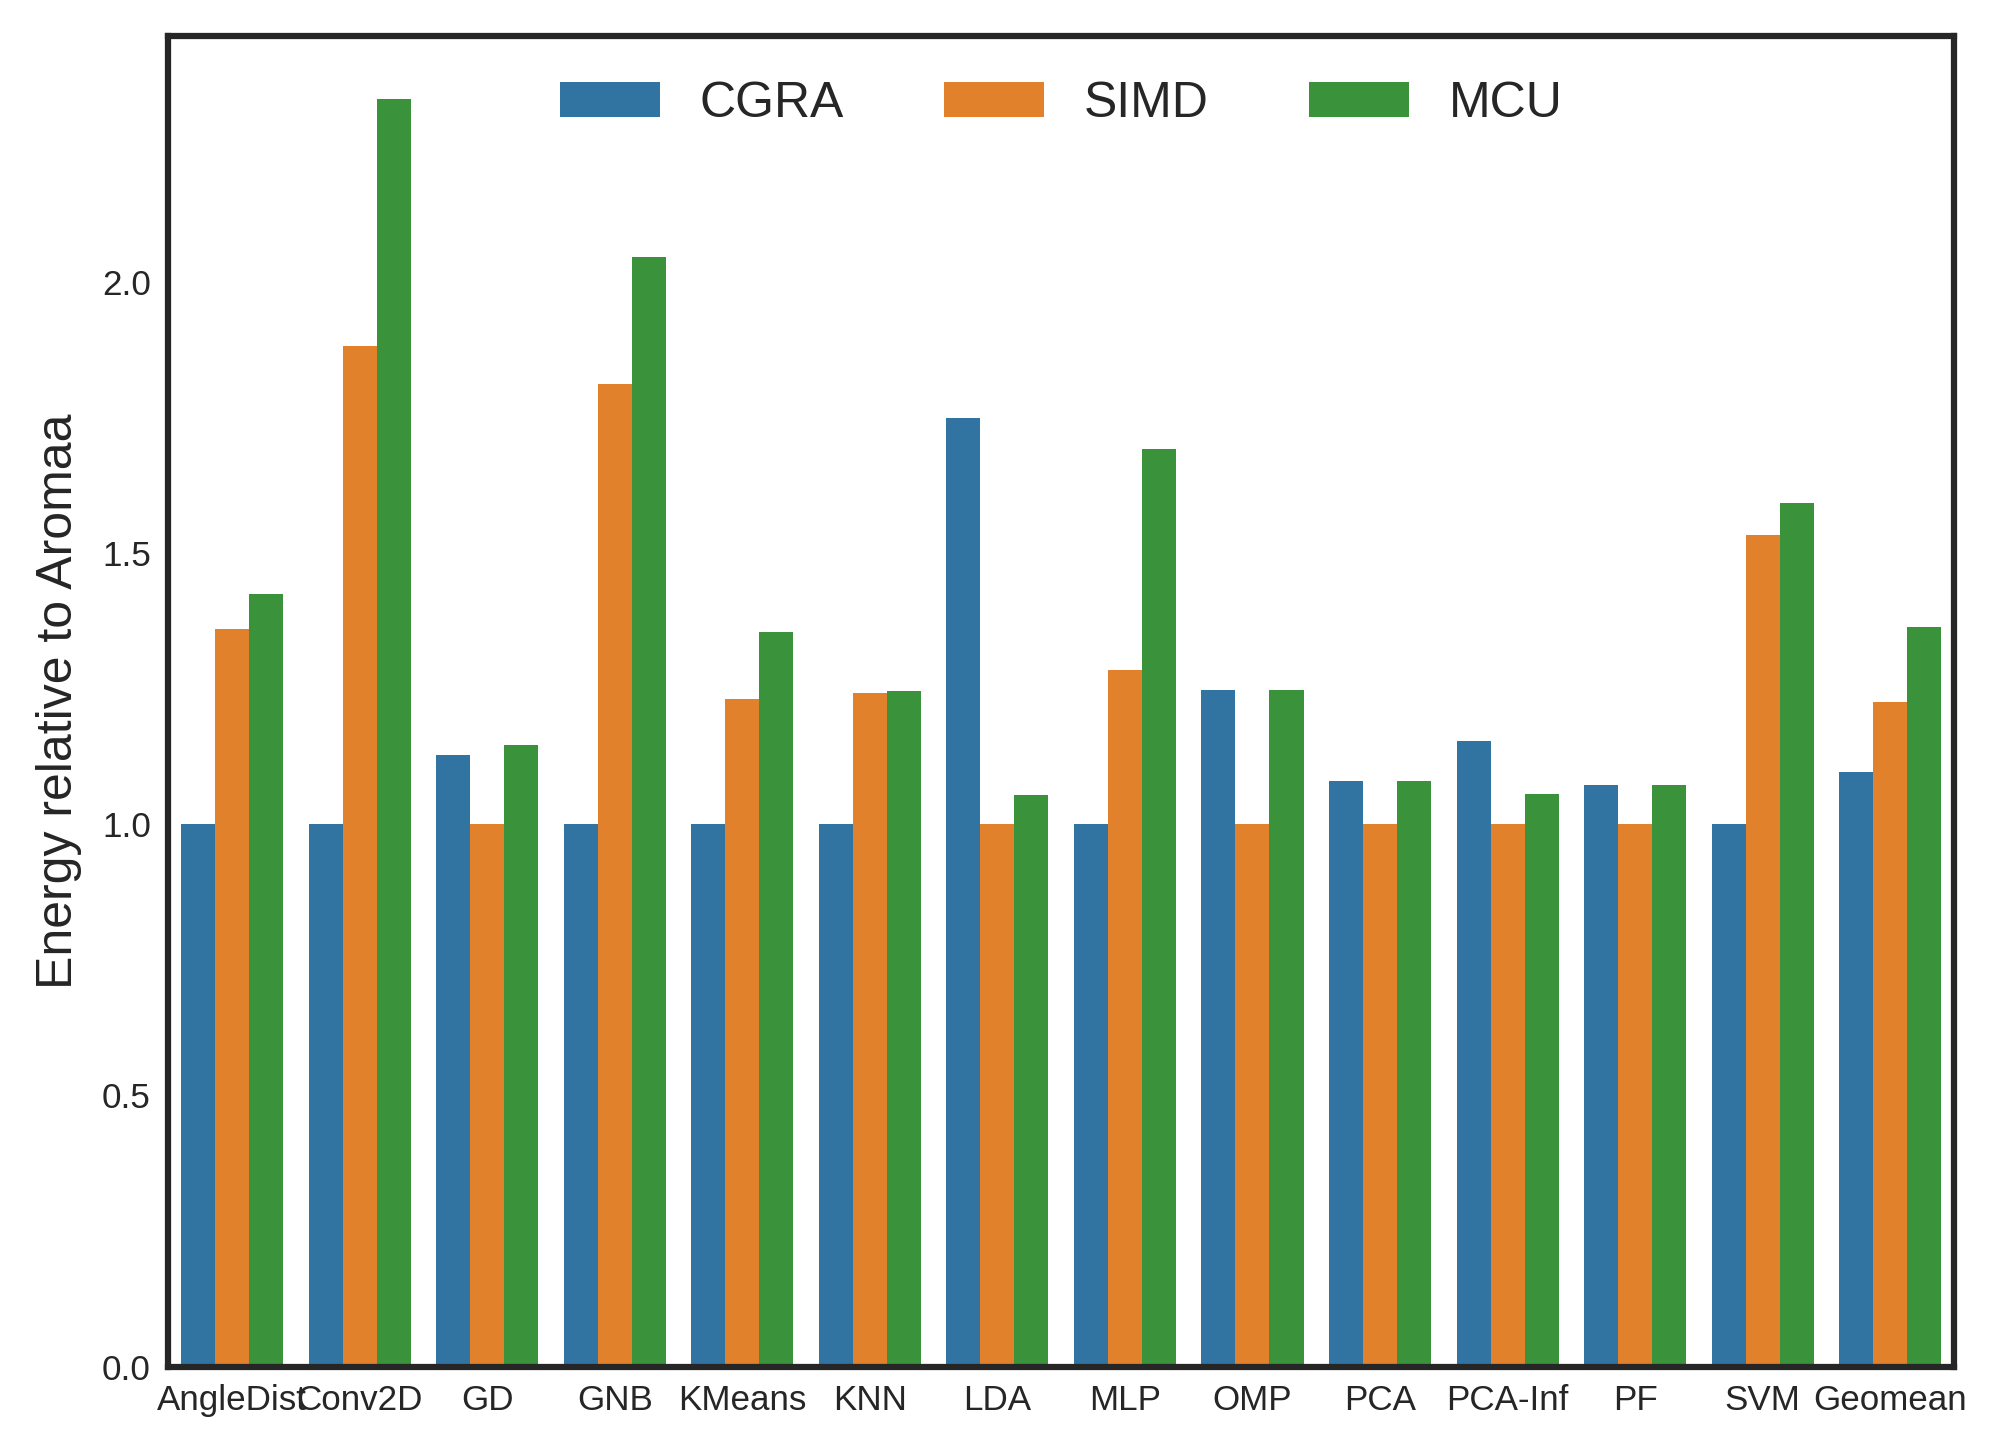
\includegraphics[width=\linewidth]{./figs/comparison_vs_baselines.png}
\caption{\small
    \arch{}'s heterogeneous design allows it to outperform an MCU, an MCU with
    SIMD, and a CGRA baseline in energy efficiency at MEOP.
}
\label{fig:vs_baselines}
\end{wrapfigure}


\subsection{Research Goals}
\label{ssec:research2}
Research objectives for \olfc{} are as follows:

\begin{enumerate}
\item Extend the representative olfactory computing applications (Sec~\ref{sec:tract2})
    into a bona fide olfactory computing benchmark suite --- NoseBench --- by
    porting all benchmark code to C and OpenMP, designing representative inputs
    for each benchmark, and providing baselines on existing systems, including
    Ahromaa; enable evaluations for heterogeneous systems --- both
    heterogeneous SoCs, as well as multi-chip and even multi-device systems.
    NoseBench --- software, data, \& build scripts --- as well as
    executable binaries for major platforms --- will be published under
    an open source license in order to enable commercial and academic
    research into \olfc{}.

    NoseBench will consist of a representative set of current and future
    \olfc{} applications.  Data and inputs will be drawn from published real
    world samples.
    
    NoseBench will be published with a CMake based build system.  As CMake
    is an open-source, cross platform build automation tool targeting all
    major operating systems, and since nearly all computer architectures
    have open source or proprietary C compilers, researchers will be able
    to get NoseBench running on a wide variety of systems quickly and easily.
    For major architectures (e.g., ARMv7, ARMv8, x86\_64, i686, etc.),
    we will provide prebuilt NoseBench binaries.
\item
    Rapid development of small and ultra-low power odor sensors means that, for
    the first time, computing power consumption may be the limiting factor
    in olfactory or chemical processing, rather than sensor power
    consumption.  In light of this development, we will perform an exploration
    of the architectural design space in order to identify good architectures
    for \olfc{} systems targeting wearable and distributed sensor networking
    olfactory applications.  Many ultra-low power candidate architectures
    currently exist, including ultra-low power microcontrollers~\cite{} and GPUs~\cite{},
    as well as \(<\si{\milli\watt}\) spatial architectures~\cite{}.
    Preliminary results analyzing olfactory applications
    and their computational requirements (Sec~\ref{ssec:prelim2}}) show that,
    for many applications, performance requirements are lax, and absolute
    computational and memory requirements are low.  This suggests that the
    architectural design space considered must go beyond looking at just
    computer organization and design, but must encompass memory design and
    operating points.

    Due to lax performance requirements and low computational requirements,
    \olfc{} is likely a strong candidate for near or sub-threshold
    computing~\cite{}.  Thus the design space exploration will include
    ammenability to and impact of voltage scaling into the near and sub-threshold
    regions.  Although this type of work has been done for CPU and GPU based
    architectures, it has, to the best of our knowledge, never been done for
    reconfigurable spatial architectures.
    
    As many \olfc{} applications require very small amounts of data memory,
        memory design will be an important aspect of the design space
        exploration.  The size, geometry, and number of SRAM banks will be
        explored.  Additionally, since some applications require trivial
        amounts of data memory, we will also consider memories composed wholy
        or partially out of latches and flip-flops, rather than SRAM cells.
        Although SRAM cells are typically smaller and consume less power than
        flip-flops and latches at nominal voltage, SRAM cells are generally not
        ammenable to voltage scaling.  Thus, at low voltages, latch and
        flip-flop based memories may consume less power than an equivalently
        sized SRAM.

\item Analyze Ahromaa and existing olfactory computing hardware in a heterogeneous, networked
     computational setting, in which computation can be offloaded from the earable
     device onto a number of other devices, including smart watches, smart phones,
     and high perfromance cloud systems;
\end{enumerate}



\section{Related Work}
There are works related to \arch{} from the perspective of low-power
design, including works on subthreshold sensor
processors~\cite{nazhandali2005energy}, other ultra low-power processors~\cite{lee2012circuit},
and architectures for energy harvester powered processors~\cite{kim2022sic}.
While parallel architectures are often thought of as having high-power, recent
works have proposed CGRAs which operate at far below nominal
frequency~\cite{gobieski2021snafu, das2017142mops}, enabling the energy
efficiency associated with dataflow architectures, while still allowing
\(\approx\si{\milli\watt}\) operations. There has also been interest in low
power SIMD architectures, including \textit{scalar} vector
processors~\cite{gobieski2019manic}, and vector processors for low-power media
applications~\cite{gebis2004viram1, nam2007low}.


SpEaC architecture
most closely resembles the SoftBrain CGRA~\cite{nowatzki2017stream} in its
architecture.  However, there are three  significant differences.
First, SoftBrain uses general purpose functional units (since it is aimed at
supporting arbitrary workloads). SpEaC replaces SoftBrain's fixed-point general
purpose functional units with fixed-point adders and multipliers - common
across our DSP and ML-based kernels.
As a result, SpEaC's functional units consume 4.42x lower power, on average,
in \SI{28}{\nano\meter} technology.
Second, SpEaC provides hardware support for complex arithmetic through support
for 2-element vectorized operations ($2\times 32$ multiplication, $2\times 32$
multiplication, $2\times 32$ addition, $2\times 32$ sub-add). SoftBrain
does not directly support complex arithmetic and, therefore, kernels such as
FFT cannot be mapped efficiently.
Third, SoftBrain uses a general purpose mesh network to support arbitrary
workloads. SpEaC replaces SoftBrain's general-purpose network with a
distribute-then-reduce tree
due to the specific multiply-add and multiply-accumulate patterns found in
earable workloads.
This provide a $4\times$ savings in CGRA network power at \SI{28}{\nano\meter}.
Overall, SpEaC consumes less than two-thirds the power of SoftBrain at
\SI{28}{\nm}.


Other related work includes MAERI~\cite{kwon2018maeri} and
SNAFU~\cite{gobieski2021snafu}. Similar to SpEaC, MAERI substrate is based on
multiply-and-add trees. However, its system architecture and programming
environment are focused on ML kernels. It is unclear how to map earable DSP
kernels such as LU, Bilinear, Cholesky, and FFT directly on MAERI. There is no
programming support for non-matrix computation (Bilinear), no hardware support
on the substrate for complex arithmetic (FFT), and no control core for running
non-multiply and add operations either (Cholesky and LU). {SNAFU integrates a
control core with a CGRA and should therefore support the earable kernels.
However, SNAFU supports a \textit{general purpose} CGRA substrate, not one
optimized for linear algebra workloads, found commonly in machine learning and
DSP applications. Unlike SpEaC, which targets linear algebraic workloads,
SNAFU's general-purpose substrate has a high ratio of multiplier-less ALU FUs
to multiplier FUs.  This means its performance for linear algebraic workloads
is multiplier limited. As a point of comparison, \cite{gobieski2021snafu}
reports SNAFU's performance on dense matrix multiply with $64\times 64$
matrices. SpEaC outperforms SNAFU on this kernel by $72\times$. While
SpEaC's \SI{1}{\giga\hertz} clock rate accounts for $20\times$ speed-up, the
additional $3.6\times$ speed-up is a result of the greater parallelism
achievable on SpEaC, due to its larger number of multipliers (16 vs 4), and
SpEaC's nearly 1-1 ratio of adders to multipliers (while SNAFU has only one
multiplier for every three adders). Similarly, while SNAFU's grid-based NoC
topology is useful for general purpose programability (since it can support
arbitrary dataflows), it consumes more power than a tree-based NoC (for
SpEaC, we estimated that the tree-based NoC is $\sim{}4\times$ lower power
than the grid-based NoC). Previous work~\cite{kwon2018maeri} has also observed
that grid-based NoCs scale poorly in power and area relative to a tree-based
NoC for the bandwidth values SpEaC targets. A direct comparison of SNAFU and
SpEaC would nevertheless be interesting once  SNAFU toolchain is made public.


\end{document}
